\chapter{The Standard Model, the Higgs Boson and New Scalar Particles}

\section{Phenomenology of the Standard Model}


The Standard Model (SM) of particle physics~\cite{Halzen:1984mc} is a description of the nature which best explain  the fundamental structure of matter and the fundamental forces which govern all known phenomena. The SM gives a quantitative description of three of the four interactions in nature: electromagnetism, weak interactions and  strong nuclear force.
Developed in the early 1970s by Glashow~\cite{GLASHOW1961579}, Weinberg~\cite{PhysRevLett.19.1264} and Salam~\cite{Salam:1968rm}, it has successfully explained almost
all experimental results and precisely predicted a wide variety of phenomena.
It is a renormalizable quantum field theory, compatible with special relativity.

\subsection*{General Picture}
The main constituents of the SM are shown in Fig.~\ref{SM}. These  are the particle  composing the ordinary matter and responsible of the forces.
\begin{figure}
\centering
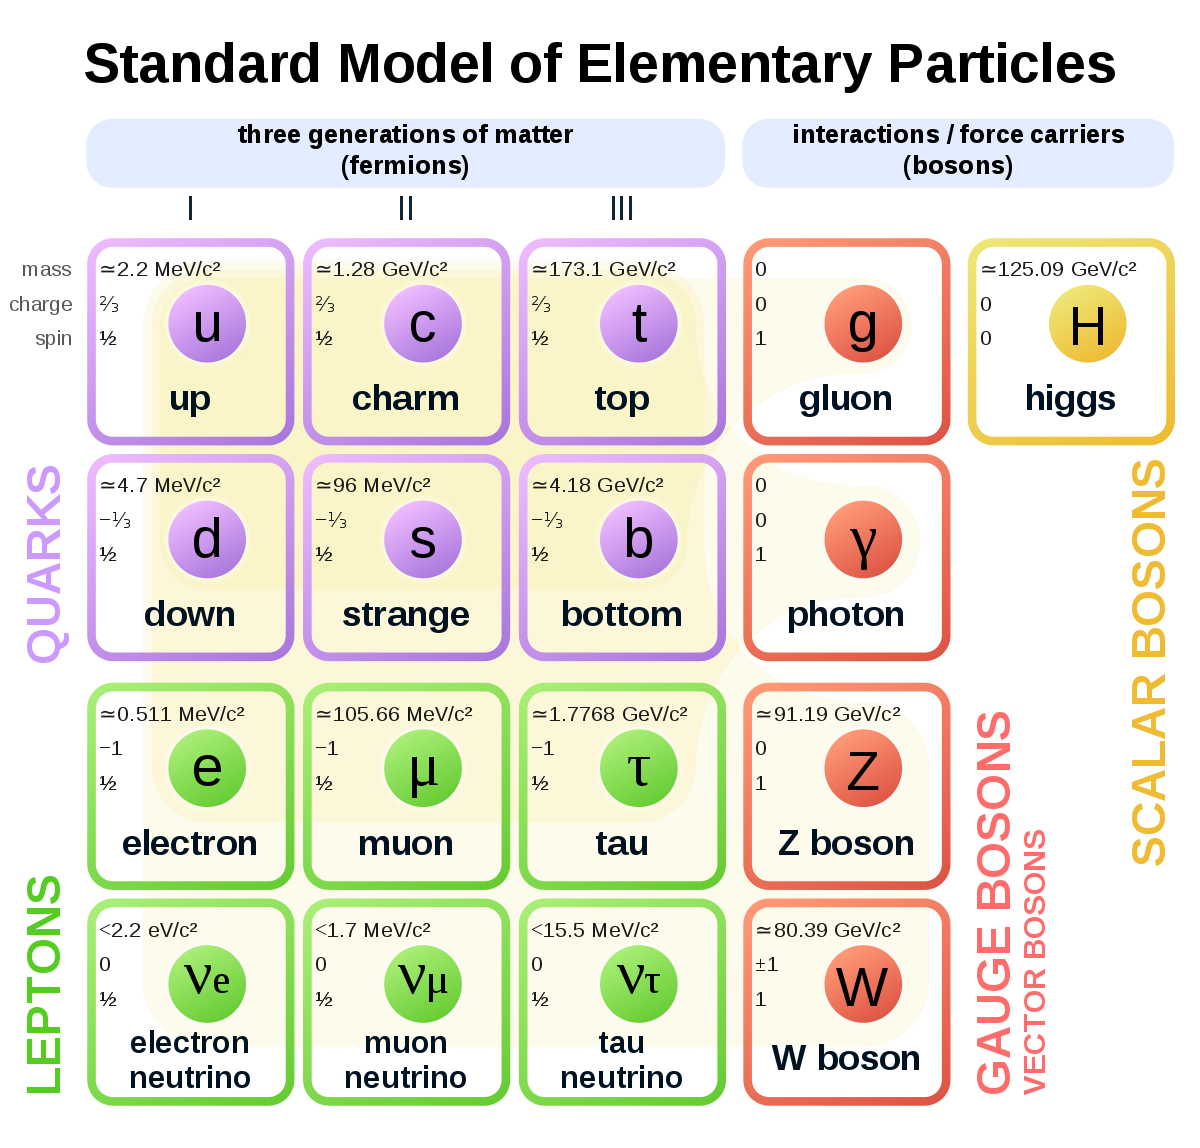
\includegraphics[scale= 0.2]{../Cap1/SM}
\caption{Main constituents of the Standard Model.}
\label{SM}
\end{figure}
The particles involved are characterized by the spin, the mass, and the quantum numbers determining their interactions.
The quarks are subject to all the three forces and, in particular, are the only fermions to
possess a ``colour'' charge, which is responsible of the strong nuclear force, as described by Quantum Chromo Dynamics (QCD). Because of the QCD colour confinement properties, quarks do not exist as free states
but can be experimentally observed only as bound states. The proton and neutron, are composed by three quarks (called baryons). The particle composed by a quark-antiquark are called ``meson''. Quark flavour is conserved in electromagnetic and strong interactions but not in weak ones, as quark mass eigenstates do not correspond to the weak interaction eigenstates.
Their mixing is described by the Cabibbo–Kobayashi–Maskawa (CKM) matrix.
The leptons have no colour charge and are subject only to the electromagnetic and weak
forces. The charged leptons of the three families are respectively denoted as the electron
(e), muon ($\mu$) and tau lepton ($\tau$). The only stable lepton is the electron. To each lepton corresponds a neutrino. The mass of neutrino is unknown but their flavour oscillations prove a non-zero mass~\cite{Balantekin:2013tqa}. 
The gluons, the W$^{\pm}$ bosons, the Z boson and the photon ($\gamma$) are boson that compose the SM gauge sector.
The gluons are the mediators of the strong interactions. They are massless, electrically neutral and carry color quantum number and they can interact with themselves.
The  W$^{\pm}$ and Z bosons are the mediator of the weak interactions. Their mass is $\sim$81 GeV and $\sim$90 GeV respectively. These particles are unstable and decay in other particles. Finally the photon is massless, chargeless, non self-interacting and mediates the electromagnetic
interactions.\\
To summarize, the SM Lagrangian may be written as the sum of three parts:
\begin{equation}
 \mathcal{L}_{SM} = \mathcal{L}_{QCD}+\mathcal{L}_{EWK}+\mathcal{L}_{H}  \:,  \end{equation}
where $\mathcal{L}_{QCD}$ is the quantum chromodynamics Lagrangian that describes the interactions of quarks and gluons, the $\mathcal{L}_{EWK}$ is the the electroweak Lagrangian that describes the interactions of the fermions with the $Z$ and  W$^{\pm}$ bosons. The $\mathcal{L}_{H}$ is the Higgs part of the Lagrangian: the Lagrangian symmetries seems to forbid the introduction of mass terms without spoiling its gauge invariance. Higgs’ proposal solves this problem by spontaneously breaking the Lagrangian symmetry (Sec.~\ref{H}).

\subsection*{Quantum Chromodynamics}
Quantum Chromodynamics describes (QCD) the interactions of quarks and gluons, mediated by
the strong force through the colour charge.  
The QCD Lagrangian has the local gauge invariance under the  $SU(3)_C$ group and it is given by~\cite{Beringer:1900zz},
\newline
\begin{equation}
\begin{split}
 \mathcal{L}_{QCD}&= \sum_q [\bar{\psi}_{q,a} ( i \gamma^{\mu} \partial_{\mu} \delta_{ab} -g_s \gamma^{\mu} t_{ab}^C A_{\mu}^C -m_q \delta_{ab})\psi_{q,b} \\
&-\frac{1}{4} F_{\mu \nu}^{A}  F^{A \; \mu \nu}] \: , \end{split}  \end{equation}
\newline
where repeated indices are summed over. The $\gamma^{\mu}$ are the Dirac $\gamma$-matrices.
The $\psi_{q,a}$ are quark-field spinors for a quark of flavor $q$ and mass $m_q$, with a color-index $a$
that runs from $a= 1$ to $N_c=R$ 3, i.e. quarks come in three ``colors''. 
Quarks are said to be in the fundamental representation of the $SU(3)$ color group. 
The $A_{\mu}^C$ correspond to the gluon fields, with $C$ running from the eight kinds of gluon.
The $t_{ab}^C$ correspond to eight $3\times 3$ matrices and are the generators of the $SU(3)_C$ group
The quantity $g_S$ is the QCD coupling constant. Finally,
the field tensor $ F_{\mu \nu}^{A}$ is given by,
\newline
\begin{equation}
 F_{\mu \nu}^{A}=  \partial_{\mu} A_{\nu}^A  - \partial_{\nu} A_{\mu}^A -g_S f_{ABC}A_{\mu}^B A_{\nu}^C  \: ,   \end{equation}
\begin{equation}
 [t^A, t^B]=i f_{ABC}t^C  \: ,   \end{equation}
\newline
where the $f_{ABC}$ are the structure constants of the $SU(3)_C$ group.
Neither quarks nor gluons are observed as free particles. Hadrons are color-singlet (i.e. color-neutral) combinations of quarks, anti-quarks, and gluons.
The fundamental parameters of QCD are the coupling $g_S$ (or $\alpha_S= \frac{g_S^2}{4\pi}$) and the quark masses $m_q$.
If the quark masses are fixed, there is only one free parameter in the QCD Lagrangian, that is $\alpha_S$. This constant is not a physical observable but
rather  a quantity defined in the context of perturbation theory, which enters prediction for experimental observable.


\subsection*{Electroweak Model}
The electroweak interactions is based on the gauge group  $SU(2)_L \otimes U(1)_Y$. 
The $SU(2)_L$ group refers to the weak isospin charge ($I$), and $U(1)_Y$ to the weak hyper-charge ($Y$). 
Left-handed ($L$) fermions are paired in $I = 1/2$ isospin doublets, whereas
right-handed ($R$) fermions in $I = 0$ singlets. The presence of these local gauge symmetries
introduces four vector bosons: three for the $SU(2)$ group, the $W_i$ fields ($i = 1, 2, 3$), and
one for $U (1)$, the B field.
This gives rise to a quantum field theory, invariant under local gauge symmetries, whose
Lagrangian is expressed as:
\newline
\begin{equation}
 \mathcal{L}_{EW}= \sum_f \bar{\psi} i \gamma^{\mu }\mathcal{D}_{\mu} \psi -\frac{1}{4} F_{\mu \nu} F^{\mu \nu}  -\frac{1}{4} \vec{E}_{\mu \nu} \cdot \vec{E}^{\mu \nu} \; ,
\end{equation}
where the sum is extended over all the fermions $f$ and where covariant derivatives which
preserve the local  gauge invariance have the following form:
\begin{equation}
\begin{split}
&\mathcal{D}_{\mu} = \partial_{\mu} +ig \vec{W}_{\mu} \cdot \frac{\vec{\tau}}{2} + i\frac{g'}{2} Y B_{\mu}   \; , \\
& F_{\mu \nu}= \partial_{\mu} B_{\nu} -\partial_{\nu} B_{\mu}  \; ,\\
& E_{\mu \nu}^{\alpha}=  \partial_{\mu} W_{\nu}^{\alpha}  \partial_{\nu} W_{\mu}^{\alpha} -g\epsilon^{\alpha \beta \gamma}  W_{\mu}^{\beta} W_{\nu}^{\gamma} \; ,
\end{split}
\end{equation}
\newline
where $\vec{\tau}$ indicates the three Pauli matrices, $g$ and $g'$ are the coupling constants which correspond respectively
to  $SU(2)_L$ and $U(1)_Y$. 
The physical fields are obtained as linear combinations of these fields:
\newline
\begin{equation}
\begin{split}
&A_{\mu}= \sin \theta_W W_{\mu}^3 + \cos \theta_W B_{\mu} \: ,\\
&Z_{\mu}= \cos \theta_W W_{\mu}^3 - \sin \theta_W B_{\mu}  \: ,\\
&W_{\mu}^{\pm}=\frac{W_{\mu}^1 \mp W_{\mu}^2 }{ \sqrt{2}} \: .
\end{split}
\end{equation}
The above equations represent two neutral particles (the photon, described by the $A_{\mu}$
field, and the $Z$ boson) and two charged particles (the $W^+$ and $W^-$ bosons). We have
further introduced the angle $\theta_W$ , which is known as the weak mixing angle or Weinberg
angle. Up to here, the theory is necessarily incomplete: all particles it describes are
massless, contradicting experimental evidence. The Lagrangian symmetries, on the other
hand, seem to forbid the introduction of mass terms without spoiling its gauge invariance.
Higgs’ proposal solves this problem by spontaneously breaking the Lagrangian symmetry.

\subsection*{Experimental evidence}
The experimental study  of the Standard Model  has made a quantum leap in the last 30 years. First of all the theory predicted the existence of W$^{\pm}$ and Z bosons in the mass range from 60 to 93 GeV~\cite{doi:10.1142/9789814644150_0006}. 
In 1976 Rubbia, Cline and McIntyre proposed the transformation of an existing high-energy proton accelerator into a proton–antiproton collider as a quick and relatively cheap way to achieve collisions above threshold for W and Z production.  This proposal  was adopted at CERN Super Proton Synchrotron (SPS) collider  and the first  proton–antiproton  collisions were collected in 1981. In the following years the W and Z bosons have been observed by UA1 and UA2 experiments with a mass of 80 GeV and 91 GeV respectively, Fig.~\ref{rubbia_f}. 
\begin{figure}
\centering%
\subfigure[]%
{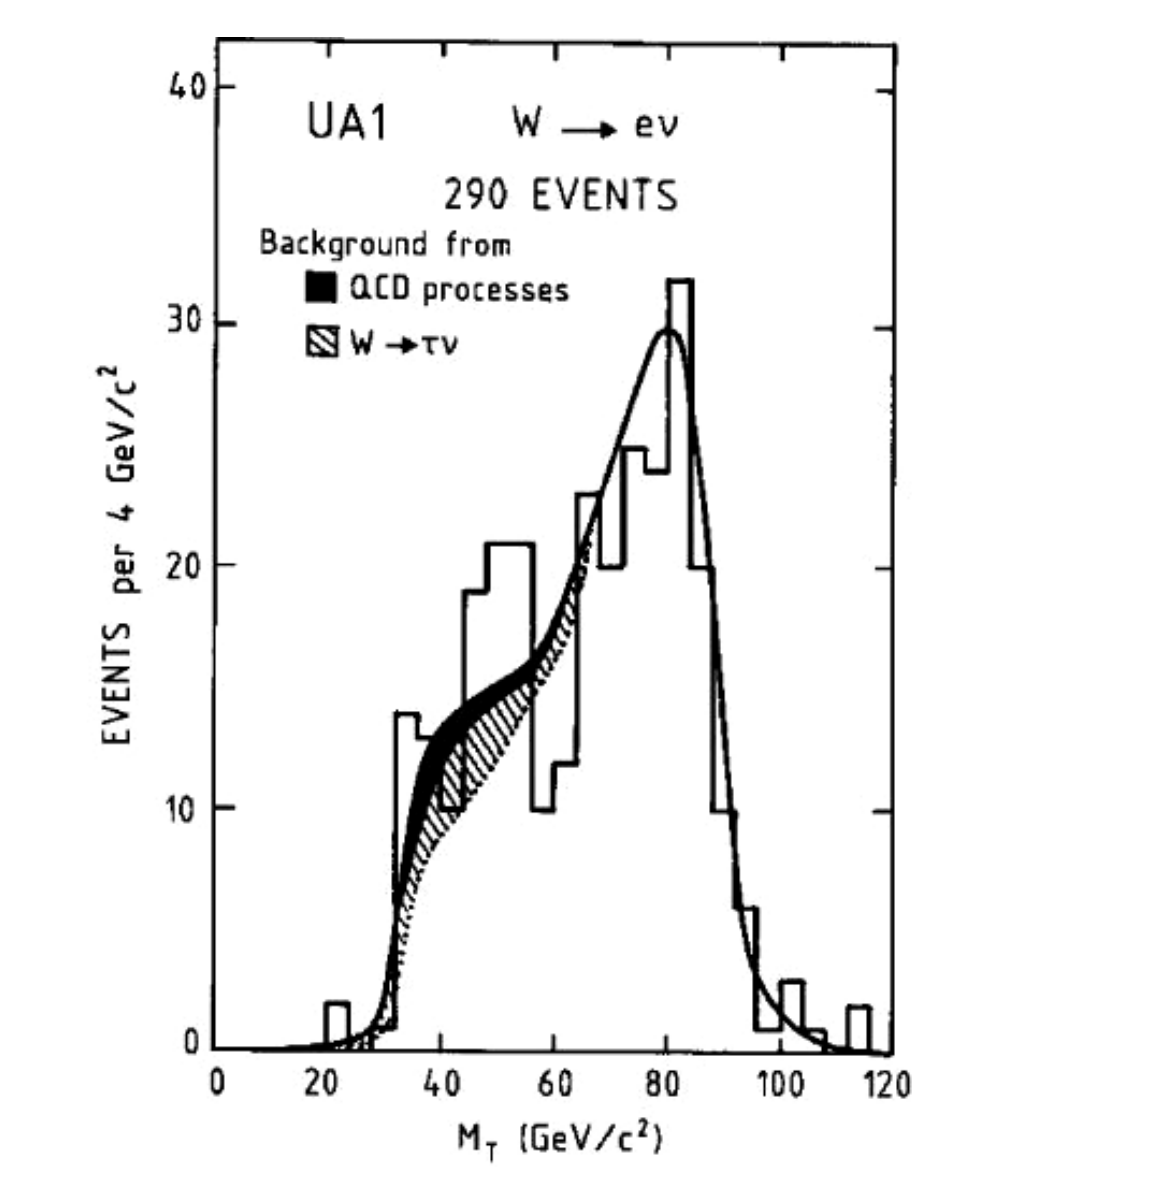
\includegraphics[scale= 0.66]{../Cap1/rubbia_W}}
\subfigure[]%
{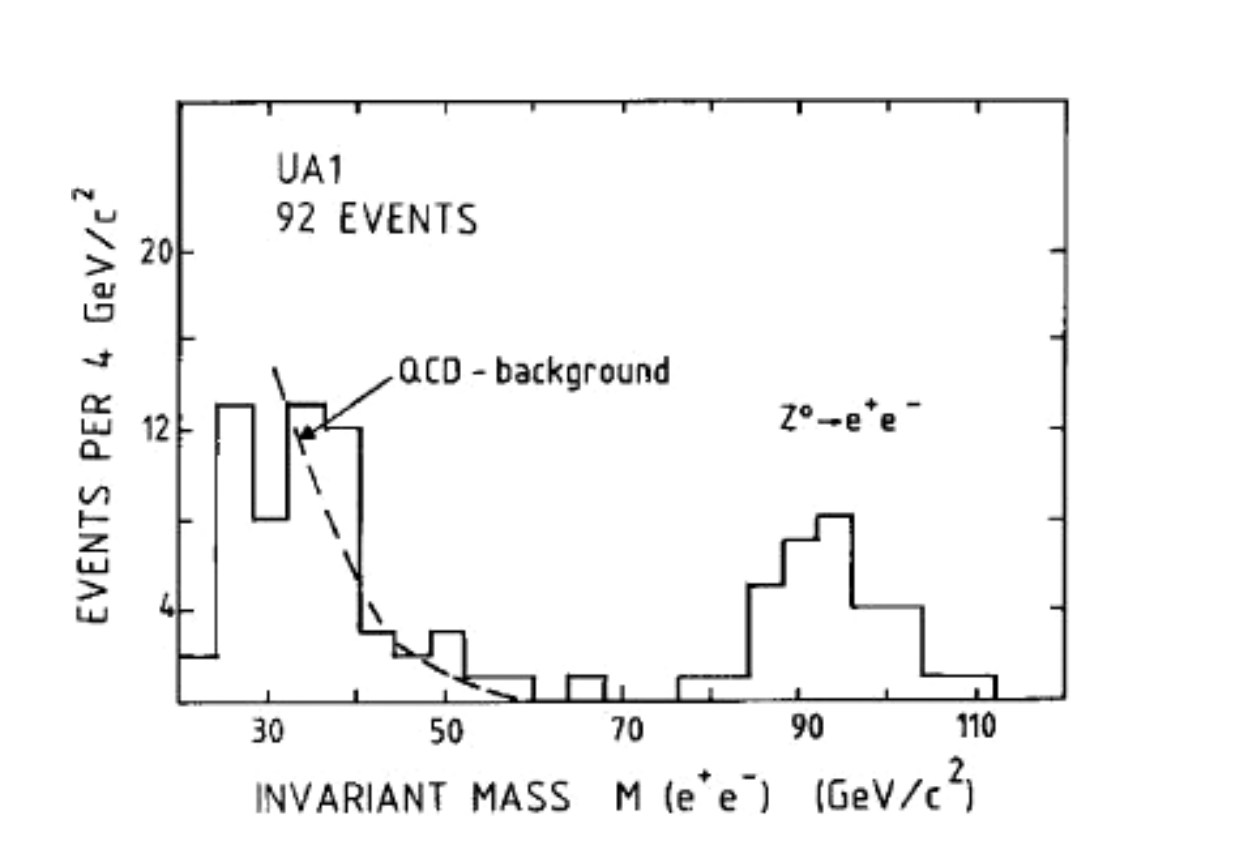
\includegraphics[scale= 0.66]{../Cap1/rubbia_Z}}
\caption{(a) Transverse mass distribution for all W$\to e \nu$ events recorded by UA1 between 1982 and 1985. (b) Invariant mass distribution of all $e^+e^-$
pairs recorded by UA1 between 1982 and 1985}
\label{rubbia_f}
\end{figure}
With the electron-positron colliders at a center-of-mass energy equal to $Z$ mass, precise measurements of the fundamental parameters of electroweak theory could be made.  In 1989, two  $e^+e^-$ colliders operation started:
the Stanford Linear Collider (SLC) at SLAC,  and the circular Large Electron
Positron collider (LEP) at CERN. Precision electroweak tests covering the measurements at the Z pole  have been conducted by SLC and LEP experiments.
W boson properties were also measured at the LEP collider, which reach 209 GeV center-of-mass energy, well above the threshold for $W^+W^-$ pair production,  Fig.~\ref{alt}. The results of measurements confirmed the SM prediction. 
\begin{figure}
\centering%
\subfigure[]%
{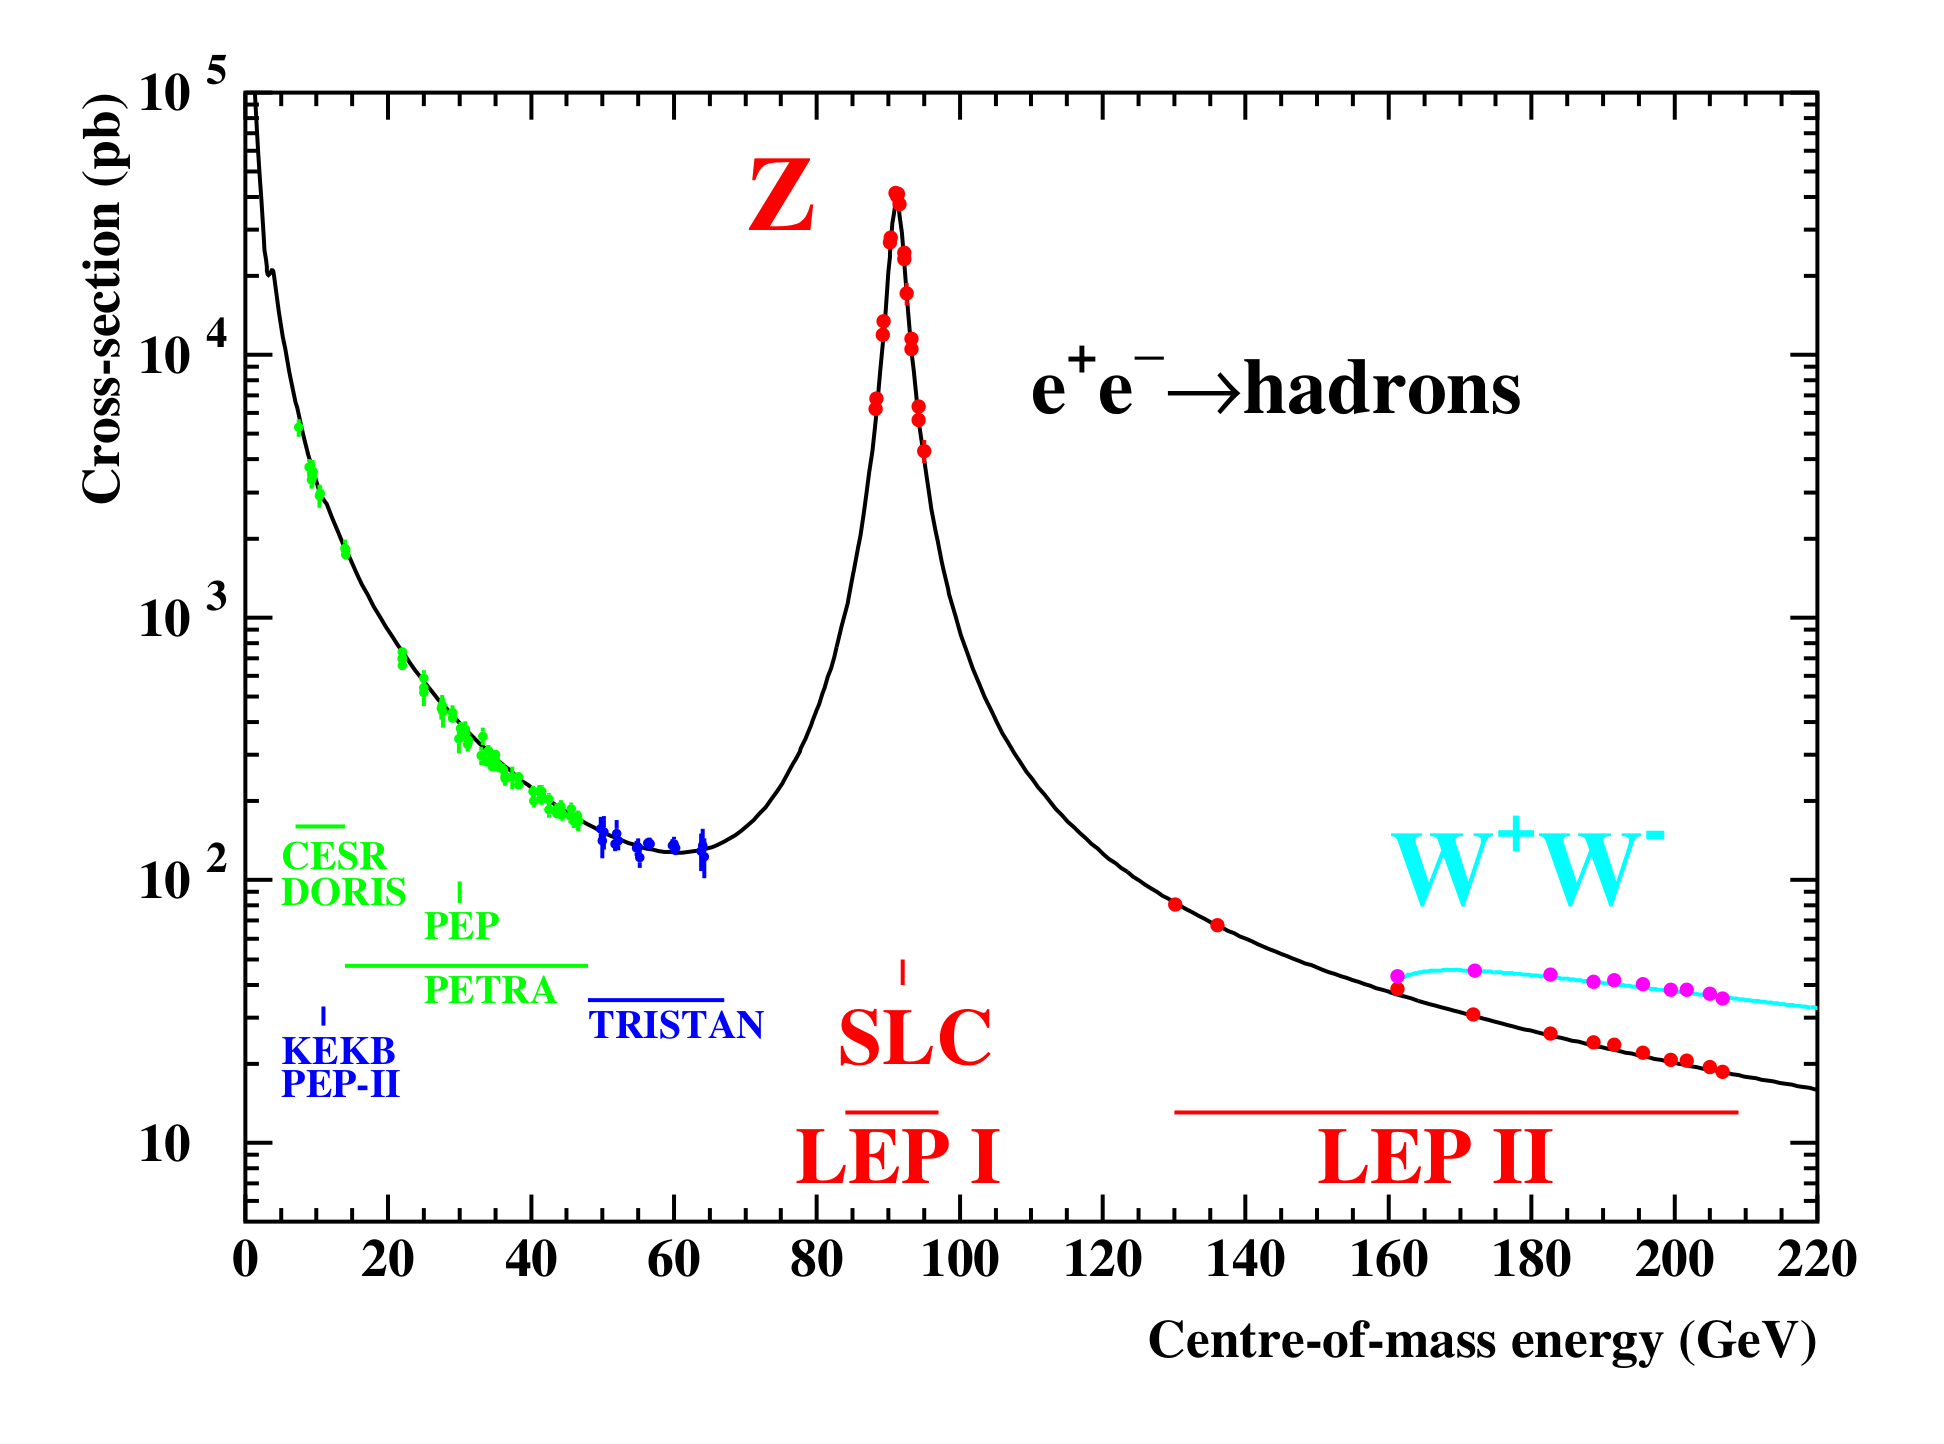
\includegraphics[scale= 0.4]{../Cap1/alt_Z}}
\subfigure[]%
{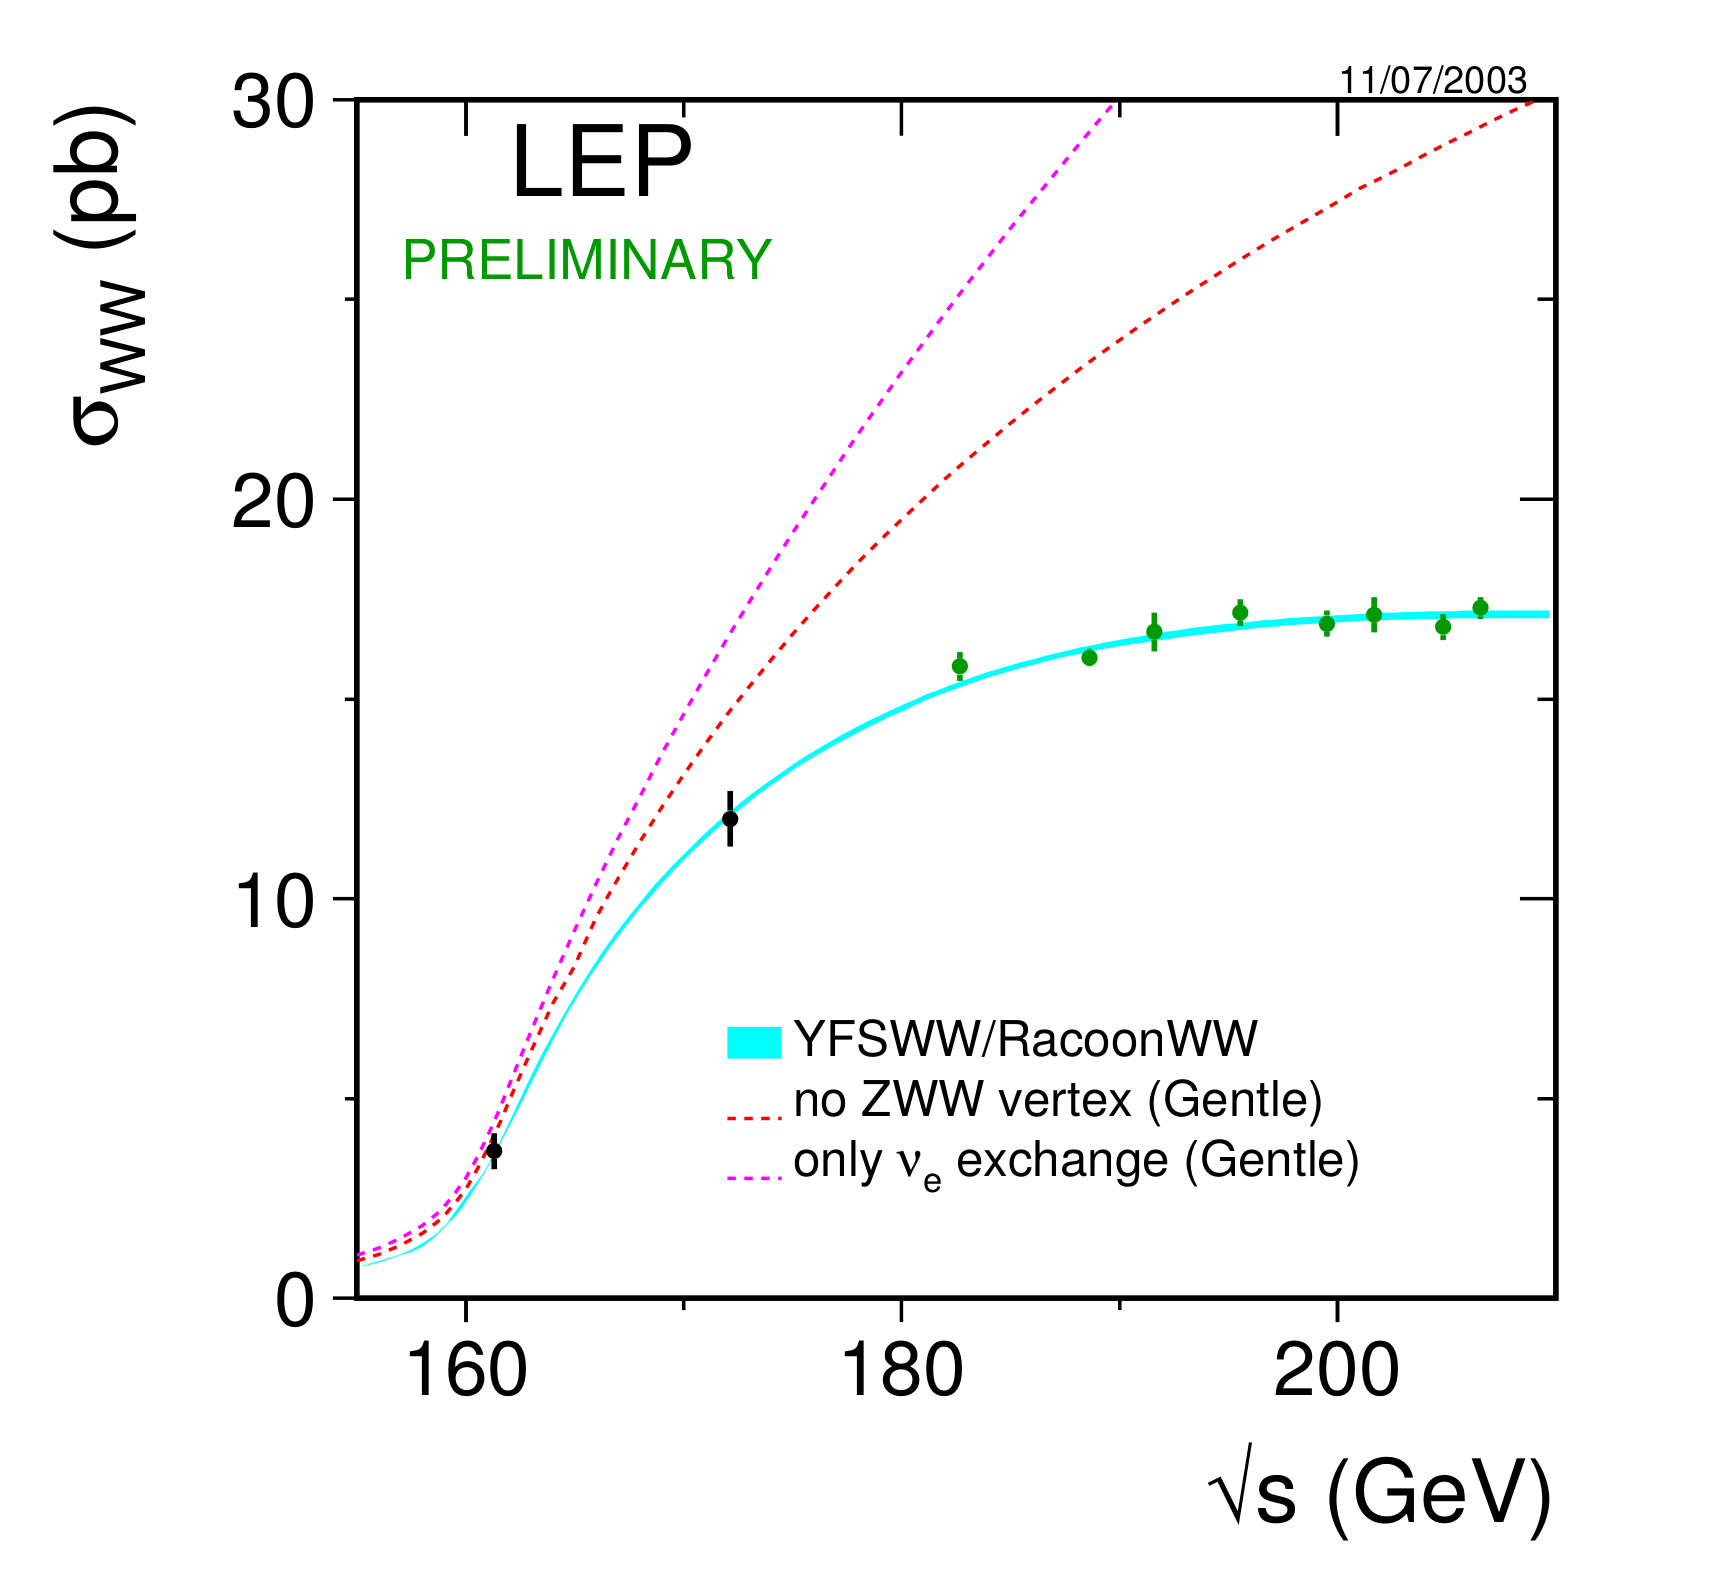
\includegraphics[scale= 0.4]{../Cap1/alt_W}}
\caption{(a) The cross-section for the production of hadrons in $e^+e^-$ annihilations. The measurements are shown as dots with error bars. The solid line shows the prediction of the SM. (b) The measured W-pair production cross section compared to the SM and alternative
theories not including trilinear gauge couplings.}
\label{alt}
\end{figure}
The next missing SM piece was top quark. It was a necessary component of the SM of electroweak interactions, but there was no consistent theoretical guidance as to what its mass should be. The only way to observe a top quark with such a high mass was at the collider with the highest-energy, the Tevatron antiproton-proton collider at Fermilab. The existence of the top quark was firmly established in 1995 with simultaneous announcements by both the CDF~\cite{PhysRevLett.73.225} and the DO~\cite{D0:1995jca} experiments with results that demonstrated a mass of around 174 GeV, Fig.\ref{Wells2004_Article_ExperimentalTestsOfTheStandard}.
After the top quark discovery, the only missing part to the SM was the Higgs boson particle  that has been observed at ATLAS and CMS experiment at LHC proton-proton collider at CERN in 2012 (see Sec.\ref{H}).  
\begin{figure}
\centering
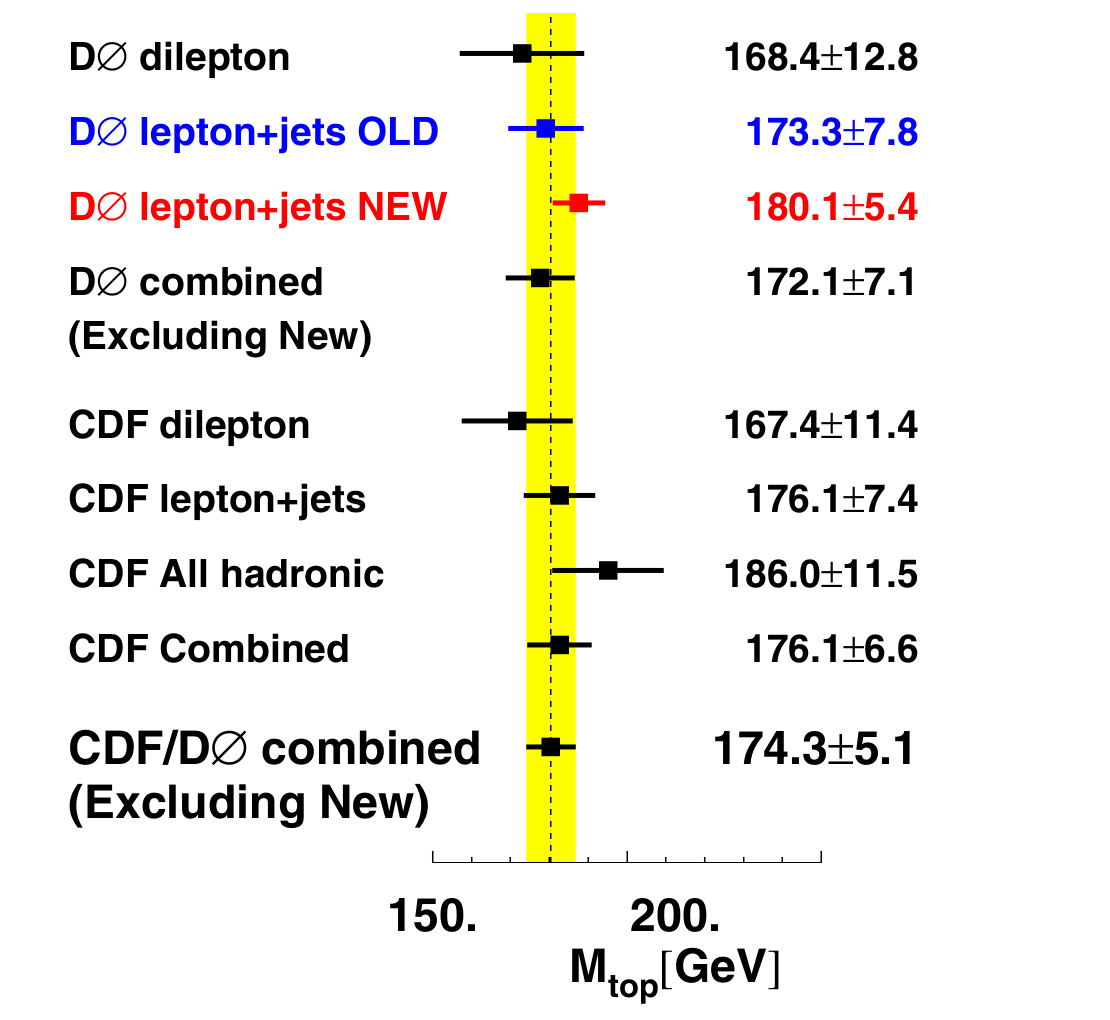
\includegraphics[scale= 0.8]{../Cap1/Wells2004_Article_ExperimentalTestsOfTheStandard}
\caption{Top quark mass measurements.}
\label{Wells2004_Article_ExperimentalTestsOfTheStandard}
\end{figure}




\section{The Higgs Boson}
\label{H}
A  Lagrangian is said to have a symmetry when it is invariant under a group of transformations. 
However the fact that the weak gauge bosons have a mass different from zero indicates that
the gauge symmetry is broken. Also the fermion masses can
not be included without violating gauge symmetry in the $\mathcal{L}_{QCD}$.
The mass terms can be introduced with the Spontaneous Symmetry Breaking Mechanism, adding  $\mathcal{L}_{H}$, that gives mass to the weak bosons and fermions and leaves the photon massless. This mechanism has been proposed in 1964 independently by Higgs~\cite{HIGGS1964132} and Brout and Englert~\cite{PhysRevLett.13.321}. With the spontaneous symmetry breaking mechanism, a  new particle which couples  to the massive fermions and to the boson emerges. This particle is called Higgs boson and its mass is a free parameter of the theory. In 2012, 48 years after this hypothesis was formulated, the Higgs boson has been observed by ATLAS~\cite{Aad:2012tfa} and CMS~\cite{Chatrchyan:2012xdj} experiments at LHC.


\subsection*{The Brout–Englert–Higgs mechanism}
The symmetry of SM Lagrangian, $\mathcal{L}_{SM}$, is $SU(2)_L \otimes U(1)_Y \otimes SU(3)_C$, where $L$, $Y$ and $C$ refers to isospin, hypercharge and color quantum numbers, respectively. To break the symmetry,  a  scalar field $\Phi$ (Higgs field) is introduced. 
The field is an  isospin doublet ($SU(2)_L$):
\newline
$$
\Phi=
\left(
\begin{array}{c}
\Phi^+   \\
\Phi^0 \\
\end{array}
\right)
=\frac{1}{\sqrt{2}}
\left(
\begin{array}{c}
\Phi_1 + i\Phi_2   \\
\Phi_3 + i\Phi_4  \\
\end{array}
\right)
$$
\newline
where $\Phi_j$ with $j=1,2,3,4$ are real fields used to manifest the complexity of $\Phi^+$ and  $\Phi^0$. The simplest Lagrangian of a self-interacting scalar field is,
\begin{equation}
 \mathcal{L}_{H}= (D^{\mu} \Phi^{\dag})(D_{\mu} \Phi) -\mu^2 \Phi^{\dag}\Phi - \lambda(\Phi^{\dag}\Phi)^2 \; , \end{equation}
where $\lambda$ needs to be positive for the potential to be bounded from below and $\mu^2$
 is a mass term for the $\Phi$ field.
The ground state (vacuum) of the theory is defined as the state where the energy density is at a minimum.
If the $\mu$ parameter is chosen so that $\mu^2<0$, the symmetry of the potential may be broken,
and  the minimum value is,
\newline
\begin{equation}
v\equiv
\sqrt{\frac{-\mu^2}{\lambda}}=\Phi^{\dag}\Phi \; .
\label{min}
\end{equation}
The choice for the sign of the
parameters $\mu^2$ and $\lambda$ gives to the potential $V(\Phi)= \mu^2 \Phi^{\dag}\Phi + \lambda(\Phi^{\dag}\Phi)^2$ the ``mexican hat'' shape, as illustrated in Fig.~\ref{higgspotential}.
\begin{figure}
\centering
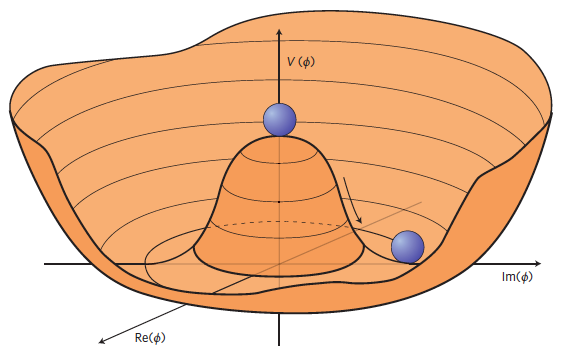
\includegraphics[scale= 0.33]{../Cap1/higgspotential}
\caption{Higgs fields potential with two degree of freedom.}
\label{higgspotential}
\end{figure}
In the perturbation theory, the $\Phi$ fields is expanded around the minimum, that is chosen among the set of states which satisfy Eq.~\ref{min}. All this states break the rotational symmetry of the Lagrangian.
The $\Phi$ field is expressed as, 
\begin{equation}
\Phi= \frac{1}{\sqrt{2}} 
\left(
\begin{array}{c}
0   \\
v +h(x) \\
\end{array}
\right) .
\end{equation}
The $h(x)$ field gives a particle with mass equal to,
\begin{equation}
m_H=\sqrt{2}\mu=v\sqrt{2 \lambda} \; ,
\label{mass_H}
\end{equation}
that is a free parameter of the theory. However some theoretical constrains could be imposed. The value of $v$ parameter in Eq.~\ref{mass_H} could be determinate by the Fermi constant, $G_F$, as,
\begin{equation}
v=\frac{2m_W}{g}=(\sqrt{2} G_F)^{-1/2} \; ,
\end{equation}
with the actual $G_F$ measurements obtained with the muon lifetime~\cite{vanRitbergen:1999fi}, a value  of~$\sim$~250 GeV is obtained for  $v$. However the  model is not predictive on the value of the $\lambda$ parameter. Nevertheless, additional theoretical arguments place approximate upper and
lower bounds on $m_H$~\cite{Beringer:1900zz}. The lower bound on the Higgs mass is given by  the vacuum state stability, that leads to requiring $\lambda$ to be
positive at all energies. The upper edge is imposed by the Planck scale. So a Higgs boson in a range of 130 $<m_H<$ 180 GeV is consistent with the theory.
 
\subsection*{The Higgs boson at LHC}
The Higgs boson  has been searched in several experiments (Fig.~\ref{650px-CMS_Higgs-event}) located  at different  colliders (LEP, SLC, Tevatron) without a clear evidence of such particle.
Therefore,  a  proton proton collider, located at CERN, that has been designed and built to Higgs boson researches specifically. 
\begin{figure}
\centering
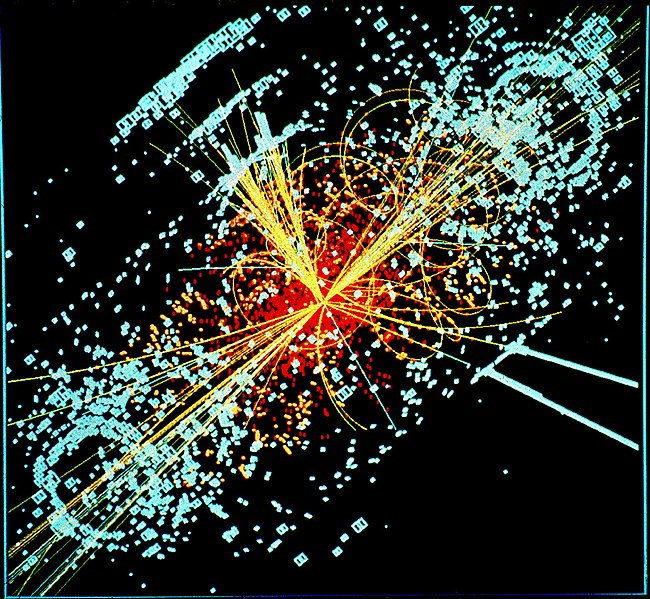
\includegraphics[scale= 0.3]{../Cap1/650px-CMS_Higgs-event}
\caption{An example of simulated data modeled for the CMS particle detector on the Large Hadron Collider (LHC) at CERN.}
\label{650px-CMS_Higgs-event}
\end{figure}  
In a proton collision the Higgs boson could be produced in different ways. The production modes are the gluon gluon fusion, the vector boson fusion (VBF), the vector-boson associated production and the top-quark associated production. Below are described the details of the different mechanisms:
\begin{itemize}
\item \textit{Gluon gluon fusion} ($gg \rightarrow H$): this is the main Higgs boson production mode. Here a couple of gluons interact via a heavy quark loop and give rise to a Higgs boson.
\begin{figure}[h]
\centering
\vspace{0.5cm}
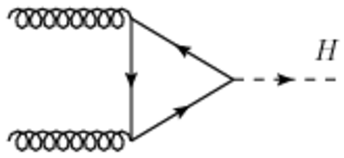
\includegraphics[scale= 0.7]{../Cap1/gg}
\end{figure}
\item \textit{Vector Boson Fusion} (VBF) ($qq \rightarrow qqH$): each incoming quarks emits a virtual W or Z boson that interact generating a Higgs boson.
The quarks after emitting the vector bosons proceed in the forward direction and represent the peculiar signature of this production mode.
\begin{figure}[h]
\centering
\vspace{1cm}
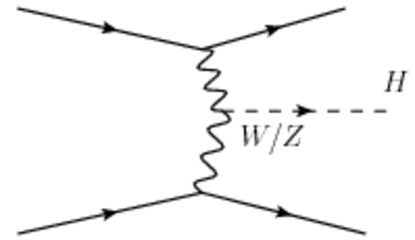
\includegraphics[scale= 0.6]{../Cap1/vbf}
\end{figure}
\item \textit{Vector boson associated production} (or \textit{Higgsstrahlung}):  the Higgs boson is emitted from a W$^{\pm}$ or a Z boson which has
been produced by a pair  quark-antiquark.
\begin{figure}[h]
\centering
\vspace{0.5cm}
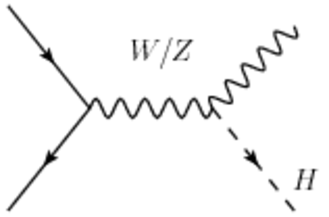
\includegraphics[scale= 0.6]{../Cap1/hlung}
\end{figure}
\item \textit{Top-quark associated production}: a pair of top quarks, originated from
the splitting of two incoming gluons, interacts to yields to a Higgs boson. 
 \begin{figure}[!htbp]
\centering
\vspace{0.5cm}
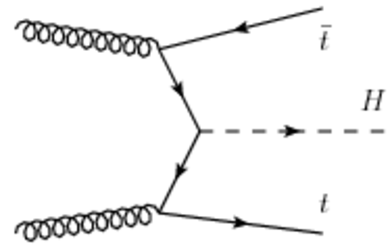
\includegraphics[scale= 0.6]{../Cap1/tt}
\end{figure}  
\end{itemize}
The Higgs boson cross section of the different production modes, depend on the center of mass energy of the collider and by the supposed mass of the particle.
The cross section increases with the energy of the colliding particles $(\sqrt{s})$ and decreases with the mass of the boson, $m_H$. The second behaviour is shown in
Fig.~\ref{prod}. The Higgs boson is an unstable particle and decays in a variety of different finale states, Fig~\ref{br}. For a Higgs boson of mass $m_H \sim$ 125 GeV (that is the mass measured by ATLAS and CMS) the channel with the largest branching ratio is in $\bar{b}b$ quark, followed by the $W^+W^-$, $\tau^+ \tau^-$ and $ZZ$ channels.

\subsection*{Experimental Results}
The discovery or exclusion of the SM Higgs boson was one of the primary scientific goals of LHC. On the 4th of July 2012, as the observation of a new boson by the ATLAS~\cite{Aad:2012tfa} and the CMS~\cite{Chatrchyan:2012xdj} collaborations has been announced, as an excess of events near 125 GeV was reported by both experiments, Fig.~\ref{disc_hig}. 
%In 2012 the proton-proton centre of mass energy was increased to 8 TeV and by the end of June an additional integrated luminosity
%of more than 5 fb$^{-1}$ had been recorded by each of these experiments, thereby enhancing significantly the sensitivity of the search for the Higgs boson.
Latest results from both the experiments confirm that  the properties of the discovered particle are consistent with the hypothesis of
being the Higgs boson predicted by the Standard Model.
\begin{figure}
\centering%
\subfigure[]%
{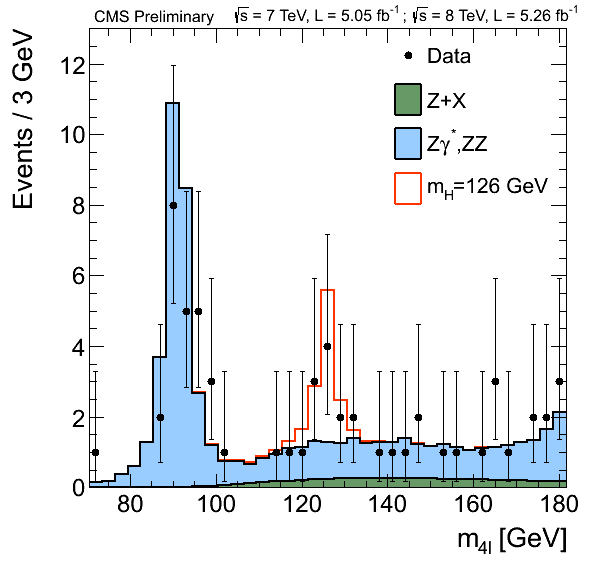
\includegraphics[scale= 0.8]{../Cap1/004}}
\subfigure[]%
{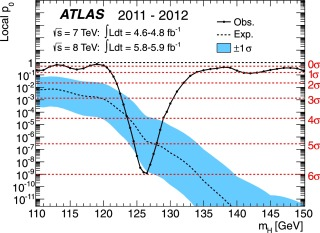
\includegraphics[scale= 0.8]{../Cap1/009}}
\caption{(a) Distribution of the four-lepton invariant mass for the ZZ$\to 4 \ell$ analysis of CMS.  (b) The observed (solid) $p_0$ local as a function of $m_H$ in the low mass range in ATLAS detector. }
\label{disc_hig}
\end{figure}
The measurements of Higgs boson couplings via exclusive production modes and decay channels, of its spin-parity, and
of its differential production cross section, need to be thoroughly investigated to verify
that they correspond precisely to the SM predictions. It is being done using the new data, collected from 2015 at LHC with  increased center-mass-energy of 13 TeV.
Precision measurements of the Higgs boson’s properties are important to understood why the Higgs
boson mass is near the electroweak scale. A good measurement that is possible to perform is the  Higgs boson's coupling. In the $k$-framework~\cite{Heinemeyer:2013tqa}  coupling modifiers are introduced in order to test for deviations in the couplings of the Higgs boson to other particles.  
Indeed, the couplings to up and down type fermions can be nonuniversal.  Additionally, in these models,
it is possible that the Higgs boson will couple differently to fermions ($k_F$) and vector bosons ($k_V$), Fig.~\ref{Figure_016}. This results so far shows a good agreement among the experimental  data and the theory.
\begin{figure}
\centering
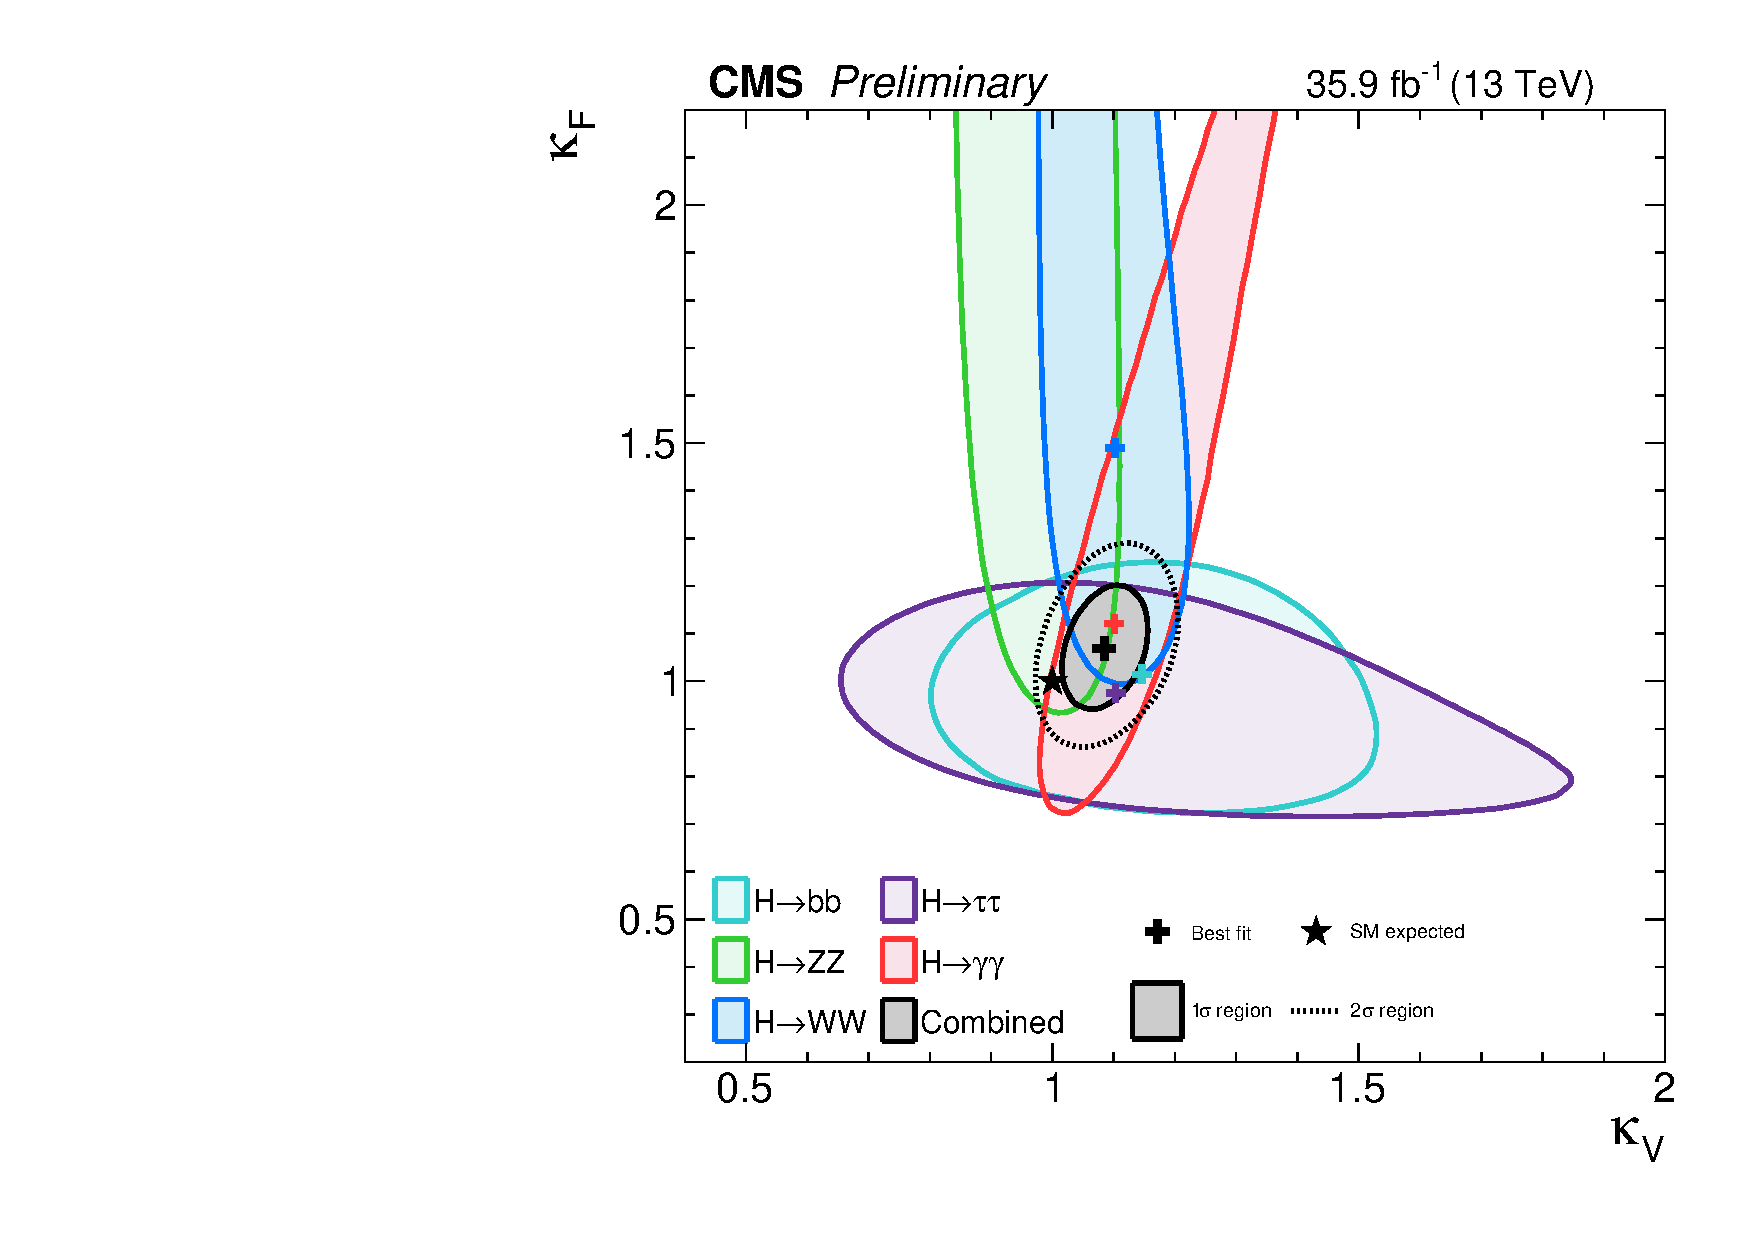
\includegraphics[scale= 0.4]{../Cap1/Figure_016}
\caption{The  CL regions in the $k_F$ vs $k_V$ parameter space for the model assuming a common scaling of all the vector boson and fermion couplings.}
\label{Figure_016}
\end{figure}  



%\subsection*{Higgs boson to WW channel}

\section{New Scalar Particles}
\label{NSP}


\subsection*{Open Questions} The Standard Model is presently the best description of the subatomic nature, but this theory does not provide a complete picture of the world. Sure enough there are still open questions: the gravity is not described in the model, the explanation of the dark matter is not clear and the  neutrino mixing and mass are not well understood.
The gravity is one of the four fundamental interactions but it is not described in the  SM. It is so different from the three other
forces. The purpose to establish a common theory that describe all forces is so difficult. The gravity is described in the  Einstein’s General Relativity (GR) theory. To combine the  SM with the GR it is necessary a quantum theory with a new field associated to gravity  as mediator: a spin 2 particle called graviton. Right now there are no experimental evidence of the existence of this kind of particle. 
An other deficit of the SM regards the dark matter. In fact, from astronomical observations, only the 5\% of the  matter and energy content of our universe is formed by the ordinary matter (hadrons and leptons), the other 95\% is composed by dark matter ($\sim$ 25\%) and dark energy ($\sim$ 70\%). The SM does not offer good candidates or explanations for the dark matter and dark energy problems although some research at colliders have been done.
Concerning the neutrinos, in the SM they were assumed massless. However flavour oscillation implies that they must have non zero mass differences.
It is not clear if the small neutrino masses  can arise from the same electroweak symmetry breaking mechanism that
is in act for the other SM particles.\\
\newline
These open questions represent  deficiencies of the Standard Model. 
The presence of a hidden sector, defined here to mean extra states that
have no SM gauge charge but are charged under some other exotic gauge symmetry, does not necessarily solve any of the problems above. However, in order to identify whether the SM Higgs sector is complete,  the searches of additional heavy scalars are performed.  They would prove the presence of beyond-the-SM (BSM) physics in the form of a non-minimal Higgs sector~\cite{Robens:2015gla}. The existence of sibling Higgs boson, denoted $X$, is motivated in many BSM scenarios, so the research in the full mass range accessible at colliders  remains one of the main objectives of the experimental community. This  program  needs  to  be continued within the full mass range that is accessible to current and future experiments.
\newline
\subsection*{Higgs Singlet Extension}
The simplest extension of the SM Higgs sector consist in adding to the complex $SU(2)_L$ doublet $\Phi$ a real scalar  $S$ which is a singlet under all SM gauge groups.  The most general gauge-invariant and renormalisable scalar Lagrangian is,
\newline
\begin{equation}
 \mathcal{L}_s = (D_{\mu} \Phi )^{\dagger}  \: D_{\mu} \Phi  +  \partial^{\mu}S   \partial_{\mu}S -V(\Phi, S)   \: ,  \end{equation}
\newline
where $V(\Phi, S) $ is the scalar potential,  
\newline
\begin{equation}
 V(\Phi, S)= -m^2   \Phi ^{\dagger}\Phi -\mu^2 S^2 +\lambda_1 (\Phi ^{\dagger}\Phi)^2 +\lambda_2 S^4 + \lambda_3 \Phi ^{\dagger}\Phi S^2 \: . \end{equation}
\newline
Here, $Z_2$ ($S \rightarrow -S$) symmetry is imposed which forbids additional terms in the potential.
To determine the condition for $V(\Phi, S)$ to be bounded from below, it is necessary to study its behaviour for large field values.
The two vacuum expectation values (VEVs) are defined as,
\begin{equation}
\langle \Phi \rangle \equiv \left(
\begin{array}{c}
0  \\
\frac{v }{\sqrt{2}}  \\
\end{array}
\right)
, \qquad 
\langle S \rangle \equiv \frac{x }{\sqrt{2}}  \:,  \end{equation}
with v and x real and non-negative.
With this definition of the VEVs, the extrema of V are determined using the following set of equations: 
\newline
\begin{equation}
\frac{\partial V}{\partial v}(v,x)= v \cdot (-m^2+ \lambda_1 v^2+ \frac{\lambda_2}{2}x^2 ) , \end{equation}
\begin{equation}
\frac{\partial V}{\partial v}(v,x)= x \cdot (-\mu^2+ \lambda_2 v^2+ \frac{\lambda_2}{2}v^2 )
\: . \end{equation}
\newline
The physically interesting solutions have $v,x>0$:
\newline
\begin{equation}
v^2=\frac{\lambda_2 m^2-\frac{\lambda_3}{2} \mu^2}{\lambda_1 \lambda_2- \frac{\lambda_3^2}{4}} \; , \end{equation}
\begin{equation}
x^2=\frac{\lambda_1 \mu^2-\frac{\lambda_3}{2} m^2}{\lambda_1 \lambda_2- \frac{\lambda_3^2}{4}} \; . \end{equation}
\newline
For the determination of the extrema we evaluate the Hessian matrix:
\begin{equation}
\mathcal{H}(v,x) \equiv \left(
\begin{array}{cc}
\frac{ \partial ^2 V}{\partial v^2} &  \frac{\partial ^2 V}{\partial v \partial x}  \\
\\
\frac{\partial ^2 V}{\partial v \partial x}   & \frac{\partial ^2 V}{\partial x^2} \\
\end{array}
\right) =     \left(
\begin{array}{lr}
  2 \lambda_1 v^2 &  \lambda_3 vx \\
\lambda_3 vx & 2 \lambda_2 x^2 \\ 
\end{array} \right) \; .\end{equation}
\newline
So, the scalar potential $V(\Phi, S)$ is bounded from below if the following conditions are fulfilled,
\begin{equation}
 4 \lambda_1  \lambda_2 - \lambda_3^2 >0   \: , \end{equation}
\begin{equation}
 \lambda_1 , \lambda_2  >0    \: , \end{equation}
where if the first condition is fulfilled, the extremum is a local minimum. The
second condition , guarantees that the potential is bounded from below for large field values.
The Higgs fields, $\Phi$ and $S$, have non-zero vacuum expectation, denoted by $v$ and $x$, respectively.
Following the unitary-gauge prescription, the Higgs fields is given by,
\newline
\begin{equation}
{\mathcal H} \equiv \left(
\begin{array}{c}
0  \\
\frac{\tilde{h}+v }{\sqrt{2}}  \\
\end{array}
\right)
, \qquad 
S \equiv \frac{h'+x }{\sqrt{2}}  \: . \end{equation}
\newline
Expansion around the minimum leads to the squared mass matrix
\newline
\begin{equation}
{\mathcal M}^2 = \left(
\begin{array}{cc}
2 \lambda_1^2 v^2 & \lambda_3 vx  \\
\lambda_3 vx & 2 \lambda_1^2 x^2 \\
\end{array}
\right)
\: , \end{equation}
\newline
with the mass eigenvalues
\begin{equation}
 m_h^2=  \lambda_1 v^2 + \lambda_2 x^2 -\sqrt{(\lambda_1 v^2 - \lambda_2 x^2)^2 +\lambda_3 (xv)^2 } \qquad,  \end{equation}

\begin{equation}
 m_H^2=  \lambda_1 v^2 + \lambda_2 x^2 +\sqrt{(\lambda_1 v^2 - \lambda_2 x^2)^2 +\lambda_3 (xv)^2 } \qquad,  \end{equation}
\newline
where $h$ and $H$ are the scalar fields of definite masses $m_h$ and $m_H$ respectively, with $m_h^2 < m_H^2$ .
The gauge and mass eigenstates are related via the mixing matrix
\newline
\begin{equation}
\left(
\begin{array}{c}
h   \\
H \\
\end{array}
\right)
=
\left(
\begin{array}{cc}
\cos \alpha & -\sin \alpha   \\
\sin \alpha & \cos \alpha \\
\end{array}
\right)
\;
\left(
\begin{array}{c}
\tilde{h}   \\
h' \\
\end{array}
\right)
\; , \end{equation}
\newline
where the mixing angle $ - \frac{\pi}{2} \leq \alpha \leq  \frac{\pi}{2} $ is given by,
\newline
\newline
\begin{equation}
\sin 2 \alpha= \frac{\lambda_3 xv}{\sqrt{(\lambda_1 v^2 - \lambda_2 x^2)^2 +\lambda_3 (xv)^2 } } \; , \end{equation}

\begin{equation}
\cos 2 \alpha= \frac{\lambda_2 x^2 - \lambda_1 v^2}{\sqrt{(\lambda_1 v^2 - \lambda_2 x^2)^2 +\lambda_3 (xv)^2 } } \; .  \end{equation}
\newline
\newline
By the  mixing matrix it is clear that the light (heavy) Higgs couplings to SM particles are now
suppressed by $\cos \alpha $ ( $\sin \alpha $).
The heavy Higgs is a new version of the SM Higgs with rescaled couplings
to the matter contents and to the gauge fields of the SM. In fact, the only novel channel
with respect to the light Higgs case is $H \rightarrow hh$. The corresponding  partial decay width, $\Gamma$, is given by \cite{Schabinger:2005ei},
\newline
\newline
 \begin{equation}
\Gamma_{ H \rightarrow hh} =  \frac{|\mu'|^2}{8 \pi m_H } \, \sqrt{1- \frac{4m_h^2}{m_H^2}}  \; , \end{equation}
\newline
where the coupling strength $\mu'$ is,
\newline
\begin{equation}
 \mu' =  - \frac{\sin 2 \alpha}{2vx} \, (\sin \alpha v + \cos \alpha x) \, (m_h^2 + \frac{m_H^2}{2})  \; . \end{equation}
\newline
In collider phenomenology, is important:
\begin{itemize}
\item the suppression of the production cross section of the two Higgs states induced by the mixing
\item the suppression of the Higgs decay modes to SM particles,
\end{itemize}
For the high mass  scenario, i.e. the case where the heavy Higgs boson is identified with the discovered Higgs state at $\sim$125 GeV, $|\sin \alpha| $= 1 corresponds to the complete decoupling of the second Higgs boson and therefore the SM-like scenario.


\subsection*{Minimal Supersymmetric Standard Model} 

With the a Higgs boson discovery, possible extensions of the Standard Model has been introduced. 
One of the simplest ways to extend the scalar sector of the SM is to add one more complex doublet to the model.
The resulting two Higgs doublet models (2HDMs)~\cite{Barroso:2013zxa} can provide additional CP-violation coming from the scalar 
sector and can easily originate dark matter candidates.  
More evolved models with additional field content have a 2HDM like scalar sector, as 
 the Minimal Supersymmetric Standard Model.  2HDMs have a richer particle spectrum with one
charged and three neutral scalars.  All neutral scalars could in principle be the scalar discovered at the LHC.\\
Two versions of the 2HDM,  one CP-conserving and the other explicitly  CP-violating, exist.    
The Yukawa Lagrangian rises  to  scalar  exchange  flavour changing neutral currents (FCNCs) that are constrained by experiments results.
A simple way to take in account the FCNCs constrains is to impose a $Z_2$ symmetry on the scalar doublets ($\Phi_{1} \to -\Phi_{1}$ and  $\Phi_{2} \to -\Phi_{2}$) 
and a corresponding symmetry to the quark field.\\
These arguments  lead four Yukawa models: types-I, types-II, types-Y (flipped) and types-X (Lepton Specific)~\cite{PhysRevD.41.3421, PhysRevD.80.015017}. 
For example, the Higgs sector of the minimal super-symmetric standard model (MSSM) is the 2HDM with a supersymmetric relation  among
the parameters of the Higgs sector, whose Yukawa interaction is of type-II, in which only
a Higgs doublet couples to up-type quarks and the other couples to down-type quarks and charged leptons.
On the other hand, a model model that tries to explain neutrino masses, dark matter corresponds to a type-X  Yukawa interaction
In this model,  the Higgs sector is the two Higgs doublets with extra scalar singlets,  in which only a Higgs doublet couples to quarks, and the other couples to leptons. Therefore it is important to experimentally determine the type of the Yukawa interaction in order to select the true model from the different predict by 2HDMs.\\
The most general Yukawa interaction under the $Z_2$ symmetry can be written as,
\newline
\begin{equation}
\mathcal{L}_{Yukava}^{2HDM} = - \bar{Q}_L Y_u \tilde{\Phi_u}u_R  - \bar{Q}_L Y_d \Phi_d d_r  -\bar{L_L} Y_l \Phi_l l_R +h.c  \; , \end{equation}
\newline
where $\Phi_f$, with $f=u,d,l$,  is either   $\Phi_1$ or $\Phi_2$. There are four independent $Z_2$ charge assignments on quarks and charged leptons, Fig~\ref{2hdm}.
\begin{figure}
\centering
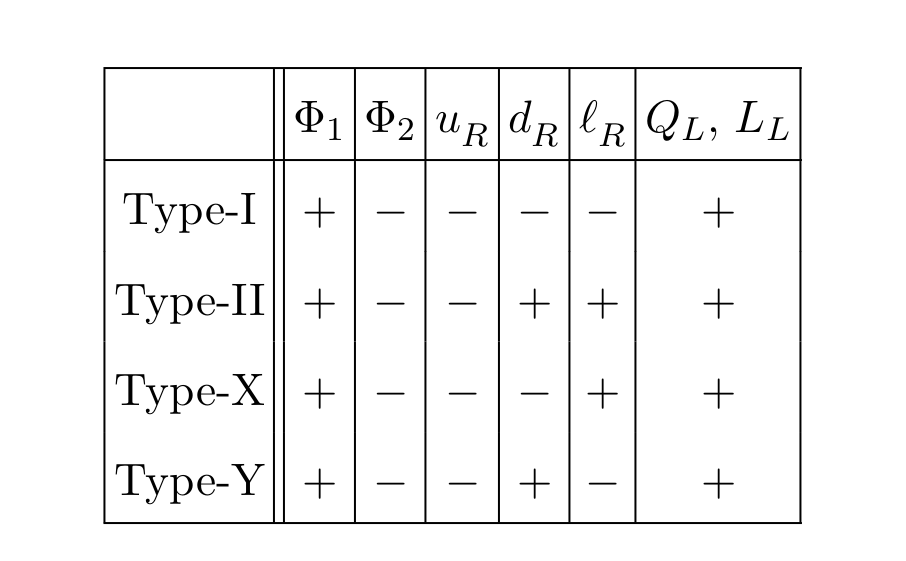
\includegraphics[scale= 0.8]{../Cap1/2hdm}
\caption{Variation in charge assignments of the $Z_2$ symmetry.}
\label{2hdm}
\end{figure}
 In the type-I, all quarks and charged leptons obtain their masses from the VEV of $\Phi_2$.  
In the type-II, masses of up-type quarks are generated by the VEV of  $\Phi_2$, while those of down-type quarks and charged leptons are acquired by that of  $\Phi_1$.The Higgs sector of the MSSM is a special 2HDM whose Yukawa interaction is of type-II. The type-X Yukawa interaction (all quarks couple to  $\Phi_2$ while charged leptons couple to  $\Phi_1$) is used in the model described in~\cite{PhysRevD.80.015017}. The remaining one is referred to as the type-Y.
The most general Higgs potential under the softly broken $Z_2$ symmetry is given by,
\newline
\begin{equation}
\begin{split}
V^{2HDM}=& m_1^2 \Phi_1^{\dag}\Phi_1 +m_2^2 \Phi_2^{\dag}\Phi_2 -m_3^2(\Phi_1^{\dag}\Phi_1 +  \Phi_2^{\dag}\Phi_2) +\frac{\lambda_1}{2}(\Phi_1^{\dag}\Phi_1)^2  \\
&+\frac{\lambda_2}{2}(\Phi_2^{\dag}\Phi_2)^2  +\lambda_3 (\Phi_1^{\dag}\Phi_1 +  \Phi_2^{\dag}\Phi_2) +\lambda_4 (\Phi_1^{\dag}\Phi_2 +  \Phi_2^{\dag}\Phi_1)  \\
&+\lambda_5 [(\Phi_1^{\dag}\Phi_2)^2 + (\Phi_2^{\dag}\Phi_1)^2] \; , \end{split} \end{equation}
\newline
where the parameters $m_3^2$ and $\lambda_5$ are complex, in general but in the following , assuming CP invariance, they are real.
The Higgs doublet fields can be parametrized as,
\newline
\begin{equation}
\Phi_i=
\left(
\begin{array}{c}
\omega_i^+   \\
\frac{1}{\sqrt{2}}(v_i +h_i+ iz_i) \\
\end{array}
\right)
\;, \end{equation}
and the mass eigenstates are defined by,
\newline
\begin{equation}
\begin{split}
\left(
\begin{array}{c}
h_1   \\
h_2 \\
\end{array} 
\right) &= R(\alpha)
\left(
\begin{array}{c}
H   \\
h \\
\end{array}
\right)\:, \qquad \\
\\
\left(
\begin{array}{c}
z_1   \\
z_2 \\
\end{array} 
\right) &= R(\beta)
\left(
\begin{array}{c}
z   \\
A \\
\end{array}
\right)\:, \qquad \\
\\
 \left(
\begin{array}{c}
\omega_1^+   \\
\omega_2^+ \\
\end{array}
\right) &= R(\beta)
\left(
\begin{array}{c}
\omega^+   \\
H^+ \\
\end{array}
\right)\:,  \end{split}
\end{equation}
\newline
where the rotation matrix is given by,
\begin{equation}
R(\theta)=
\left(
\begin{array}{lr}
\cos \theta & -\sin \theta   \\
\sin \theta & \cos \theta  \\
\end{array}
\right)
\;. \end{equation}
There are five physical Higgs bosons,  i.e., two CP-even states $h$ and $H$, one CP-odd state $A$
, and a pair of charged states $H^{\pm}$, and $z$ and $\omega^{\pm}$ are Nambu-Goldstone bosons that are eaten as the longitudinal components of the massive 
gauge bosons. The eight parameters, $m_i^2$ ($i=1,3$) and $\lambda_j$ ($j=1,5$) in the Higgs sector are replaced by eight physical parameters:
\begin{itemize}
\item the VEV $v=\sqrt{v_1^2+ v_2^2} \sim 246$ GeV,
\item the mixing angles $\alpha$ and $\beta$ ($\tan \beta= v_1/V_2 $) with $\sin( \beta -\alpha)=1 $,
\item boson masses, $m_h, m_H,m_A,m_H^{\pm} \:$,
\item  soft breaking mass parameter, $M=m_3/\sqrt{\sin \beta \cos \beta}$.
\end{itemize}
For the successful electroweak symmetry breaking, a combination of quartic coupling constants should satisfy the condition of vacuum stability.
In addition it is also take into account
bounds from perturbative unitarity to restrict parameters in the Higgs potential.
The top and bottom Yukawa coupling constants cannot be taken to
o large. The requirement $|Y_{t,b}< \pi|$  at the tree level can provide a milder constraint $0.4 <\tan \beta <91$.\\
The  wide  range  of  possibilities  for  Higgs  boson  mass  spectrum  hierarchies  and  branching
ratios  in  2HDMs  yields  a  diversity  of  production  and  decay  channels  that  are  relevant  for
multi-lepton  signatures  at  the  LHC.  Multi-lepton  final  states  become  especially  important
when the decay of one Higgs scalar to a pair of Higgs scalars or a Higgs scalar and a vector
boson is possible. 



\subsection*{The $WW$ channel for high mass particle}
Let’s now concentrate on the $X \to WW$ channel, that is the  final state using in the following  for the high mass searches.
The two dominant production mechanisms of high mass SM-like Higgs boson are the
gluon gluon fusion and Vector Boson Fusion,  Fig. \ref{prod}. 
The first one is the main mechanism for mass values below 1 TeV, above the VBF production mechanism become more and more important as $m_X$ increases.
\begin{figure}
\centering
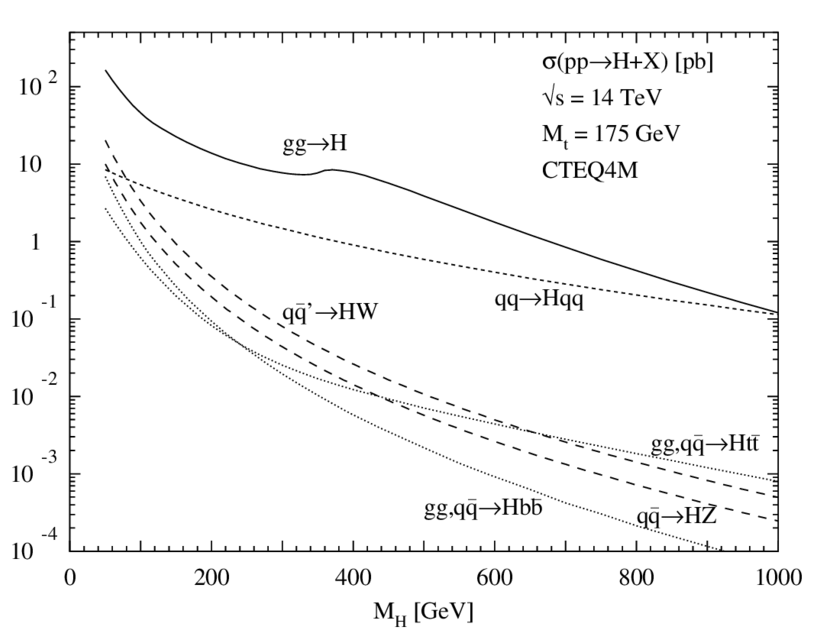
\includegraphics[scale= 0.4]{../Cap1/Higgs-production-cross-sections-at-the-LHC-for-various-production-mechanisms-as-a}
\caption{Higgs-production cross sections at the LHC for various production mechanisms as a function of the Higgs mass. QCD corrections are included except for Higgs bremsstrahlung~\cite{Djouadi2004}.}
\label{prod}
\end{figure}
In the search for high mass Higgs boson, in many models, the WW final state, along with ZZ, is the dominant decay channel of $X$ for masses above $2m_Z$ threshold. This fact is evident in Fig.~\ref{br}~(a), where the $WW$ branching ratio (in green) dominates in the high mass region. More detailed results on the decays $H \to WW$ and $H \to ZZ $ with the subsequent decay chain are presented in Fig.~\ref{br}~(b).
However even if the yield for the decay channels started by the $X \to WW$ decay is higher,  the
presence of neutrinos in the final state does not allow to have a complete reconstruction of the decay.
 This fact makes this channel very challenging. 
As we have already noticed, gluon gluon fusion cross section  is between one
and two orders of magnitude larger than that of VBF for a wide range of Higgs masses.
Nevertheless, the VBF becomes competitive when the mass approaches to 1 TeV. 
Furthermore, in case of gluon gluon production mechanism, in addition to the two lepton and two neutrinos, there are rarely one or more jets coming from initial state radiation, Sec.~\ref{ps}. 
The VBF production, providing two more jets (the VBF jets coming from the hadronization quarks from production) to the final
state, benefits from a highly reduced background with respect to the gluon gluon production mode,
such that even if the VBF production mechanism has a branching ratio smaller than the
gluon-gluon fusion, a higher signal-to-noise ratio is expected.
\begin{figure}
\centering%
\subfigure[]%
{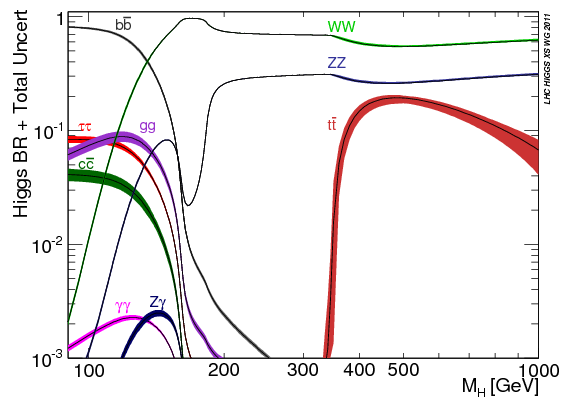
\includegraphics[scale= 0.4]{../Cap1/plots_decay}}
\subfigure[]%
{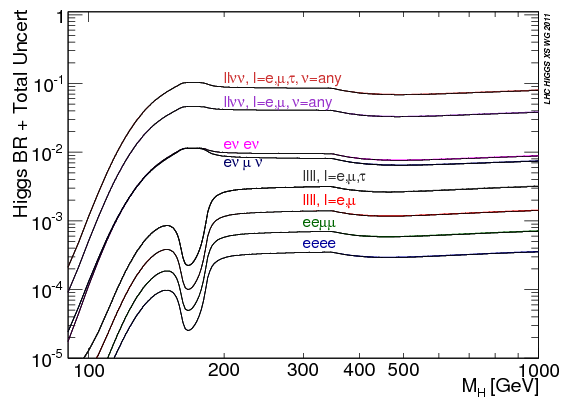
\includegraphics[scale= 0.4]{../Cap1/BRTotalUncertBands4f}}
\caption{(a) Higgs branching ratios and their uncertainties for the full mass range~\cite{Denner:2011mq}. (b) Higgs branching ratios for the different $H \to 4 \ell$ and $H \to 2\ell 2\nu $ final states and their uncertainties for the full mass range~\cite{Denner:2011mq}.}
\label{br}
\end{figure}



\subsection*{$X \to WW$ searches at colliders}
The search of high mass particle with  $WW$ final state  has been widely performed at experiments at hadron
colliders to search for new particles beyond the SM. 
The resonant $WW$ production has been studied at both the Fermilab Tevatron Collider, and the CERN Large
Hadron Collider, with the progressively increasing energy collision and integrated
luminosity. Each machine in its time has therefore probed the highest masses of
 resonances accessible. A review of the different searches
performed by D0, CDF, ATLAS and CMS, their techniques, data, results, and
limits on new particles decaying to $WW$ are described. 

\paragraph{Searches at Tevatron} Before the Higgs boson discovery, the mass  searches for the high masses SM-like Higgs boson has been performed at the CDF
and D0 detector, being the Higgs boson mass a free parameter. 
These searches result in exclusions of the high mass range  156.5 $<m_H<$173.7 GeV for CDF and 161$<m_H<$170 GeV for D0~\cite{Petridis:2012jd}. 
The high mass searches at CDF and D0 require at least one electron or a muon in the final state in order to suppress the QCD background. Given this requirement all possible decay  modes  are  considered  to  maximise  the  signal  acceptance. The di-lepton plus missing transvere energy channel requires two electrons or muons (plus neutrinos) of opposite charge in the final state. This represents a small WW decay branching ratio, but a clean signature offering the highest sensitivity  of  all  the  high  mass  channels. 
CDF and D0 set limits by combining all of the SM high mass channels with up to 8.2 fb$^{-1}$of integrated luminosity, Fig~\ref{tevatron}.

\begin{figure}
\centering
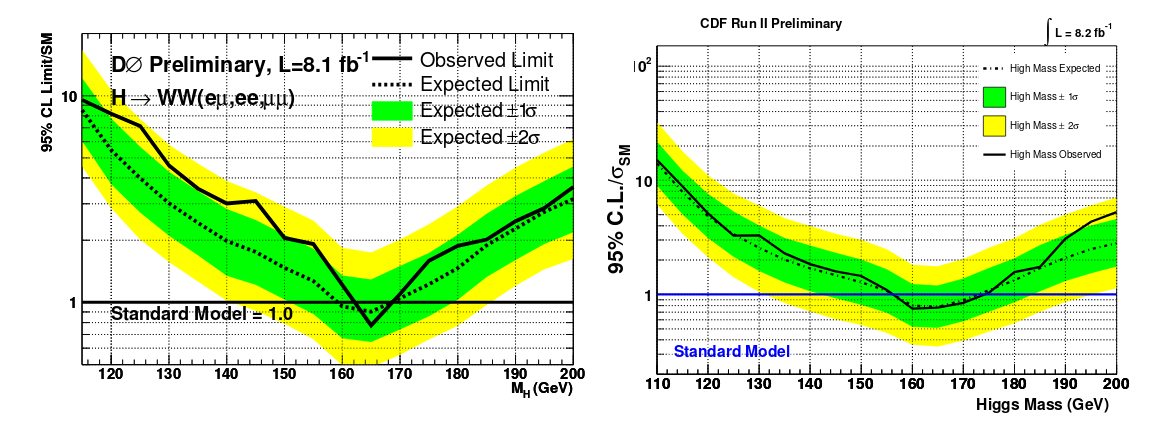
\includegraphics[scale= 0.33]{../Cap1/tevatron}
\caption{Combined limits using the di-lepton channels for D0 (left) and CDF (right).}
\label{tevatron}
\end{figure}

\paragraph{Searches at LHC} After the discovery of the Higgs boson at LHC, the two experiments, ATLAS and CMS, have been focused on high mass searches using the data collected at $\sqrt{s}=$7, 8 (Run-I) and 13 TeV (Run-II). A search for a heavy Higgs boson in the $H \to WW$ and $H \to ZZ$ decay channels has been performed by the
CMS experiment based on  proton-proton collision data samples corresponding to an integrated luminosity of up to 5.1 $fb^{-1}$ at $\sqrt{s}=7$ TeV and up to 19.7  $fb^{-1}$ at $\sqrt{s}=8$~\cite{Khachatryan:2015cwa}. This analysis is performed in a mass range 145 < $m_H$ < 1000 GeV and searches for a heavy Higgs boson in the EW singlet extension of the SM. The peculiarity of this analysis is that the full Run-I statistics is considered and the mass range reach 1 TeV for the first time in CMS.
In the case of a high Higgs boson decaying into a pair of W bosons, the fully leptonic ($X \to WW \to 2\ell 2\nu$) and semileptonic ($X \to WW \to \ell \nu qq$) final
states are considered in this  analysis. 
Decays containing four charged leptons  ($X \to WW \to 2\ell 2\ell'$), two charged leptons and two quarks ($X \to ZZ \to \ell \nu qq$) and two charged leptons and two neutrinos ($X \to ZZ \to 2\ell 2\nu$) are considered. No significant excess over the expected
SM background has been observed and exclusion limits have been set. The combined results obtained for a heavy Higgs boson with SM-like couplings for all
the different contributing final states are displayed in Fig.~\ref{plots_combination_combinedSM_def}. On the left, the observed
95\% CL limit is shown for each final state. On the right, the expected and observed limits are
displayed for each of the individual channels as well as the combined result.
\begin{figure}
\centering
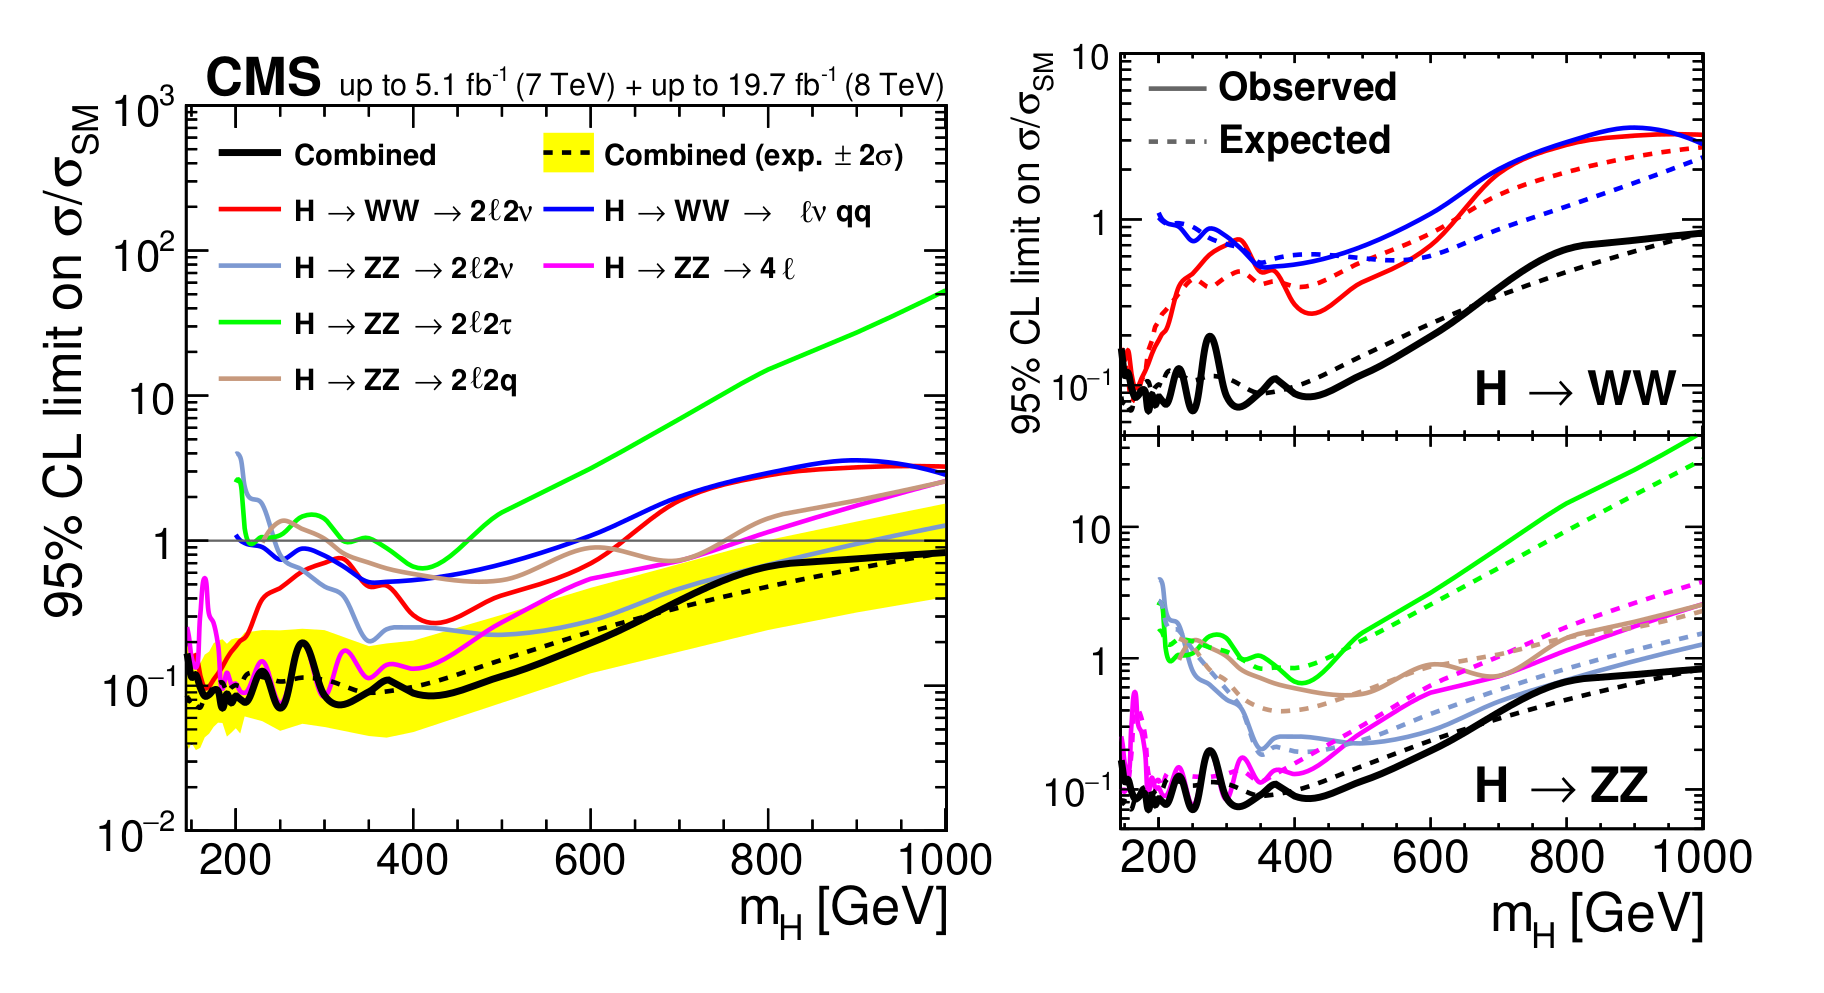
\includegraphics[scale= 0.9]{../Cap1/plots_combination_combinedSM_def}
\caption{Upper limits at the 95\% CL for each of the contributing final states and their combination. }
\label{plots_combination_combinedSM_def}
\end{figure}
Using the 13 TeV proton-proton collision data produced at the LHC in 2015, corresponding to an integrated luminosity
of 2.3 fb$^{-1}$, CMS has  performed the search for a final state with different flavour leptons ($X \to WW \to 2\ell 2\nu$) in the mass range  200$< m_H< 1000$ GeV~\cite{CMS-PAS-HIG-16-023}. The search has been carried out in the 0-jets, 1-jet and VBF categories in order to increase the signal sensitivity to different production mechanisms and maximize the exclusion limits. 
No significant excess with respect to the SM background expectation has been observed, and
the exclusion limits on the cross section times branching ratio to  $ WW \to 2\ell 2\nu$ ave been reported, Fig.~\ref{lim_2015}
\begin{figure}
\centering
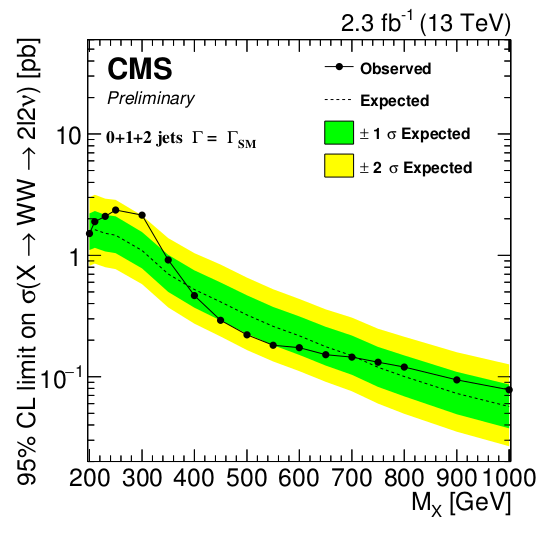
\includegraphics[scale= 0.4]{../Cap1/lim_2015}
\caption{Expected and observed exclusion limits at 95\% CL on the sum of ggH and VBF cross
sections times branching fraction for the combination of the three jet categories as a function
of the resonance mass. The black dotted line corresponds to the central value while the yellow
and green bands represent the $\pm 1\sigma$ and $\pm 2\sigma$  uncertainties respectively. }
\label{lim_2015}
\end{figure}
The ATLAS collaboration published the results of a search for a heavy neutral scalar decaying to two $W$ bosons using the datasets collected in 2015 and early
2016 at a centre-of-mass energy $\sqrt{s}=$13 TeV corresponding to an integrated luminosity of 13.2 fb$^{-1}$ in the mass range between
300 GeV and 3 TeV~\cite{ATLAS-CONF-2016-074}. In this analysis, categories with one- and at least two-jets
are optimised for a vector boson fusion-like signal and the remaining category is quasi-inclusive
for a gluon gluon fusion-like signal. The search sensitivity depends on the assumed Higgs boson width. Two different hypotheses are tested:
a narrow width approximation, where the width of the heavy Higgs boson is smaller than the
experimental resolution, and a large width assumption, where widths of 5\%, 10\%, and 15\% of
the heavy Higgs boson mass are considered.
Upper limits are set on  the production cross section times the $H \to WW$ branching ratio in two scenarios:
a high-mass Higgs boson with a narrow width, and  with intermediate widths (of 5, 10, 15\% of the
heavy Higgs boson mass), Fig.~\ref{ATLAS-CONF-2016-074_fig}. Values above 4.3 pb (1.4 pb) at $m_H=$300 GeV (400 GeV) and above 0.051 pb
(0.071 pb) at 3 TeV are excluded at 95\% CL by the gluon gluon fusion quasi-inclusive NWA (LWA 15\%) analysis. For
the VBF NWA case, the upper exclusion limit ranges between 1.1 pb at $m_H=$ 300 GeV to 0.03 pb at 3 TeV.

\begin{figure}
%\centering
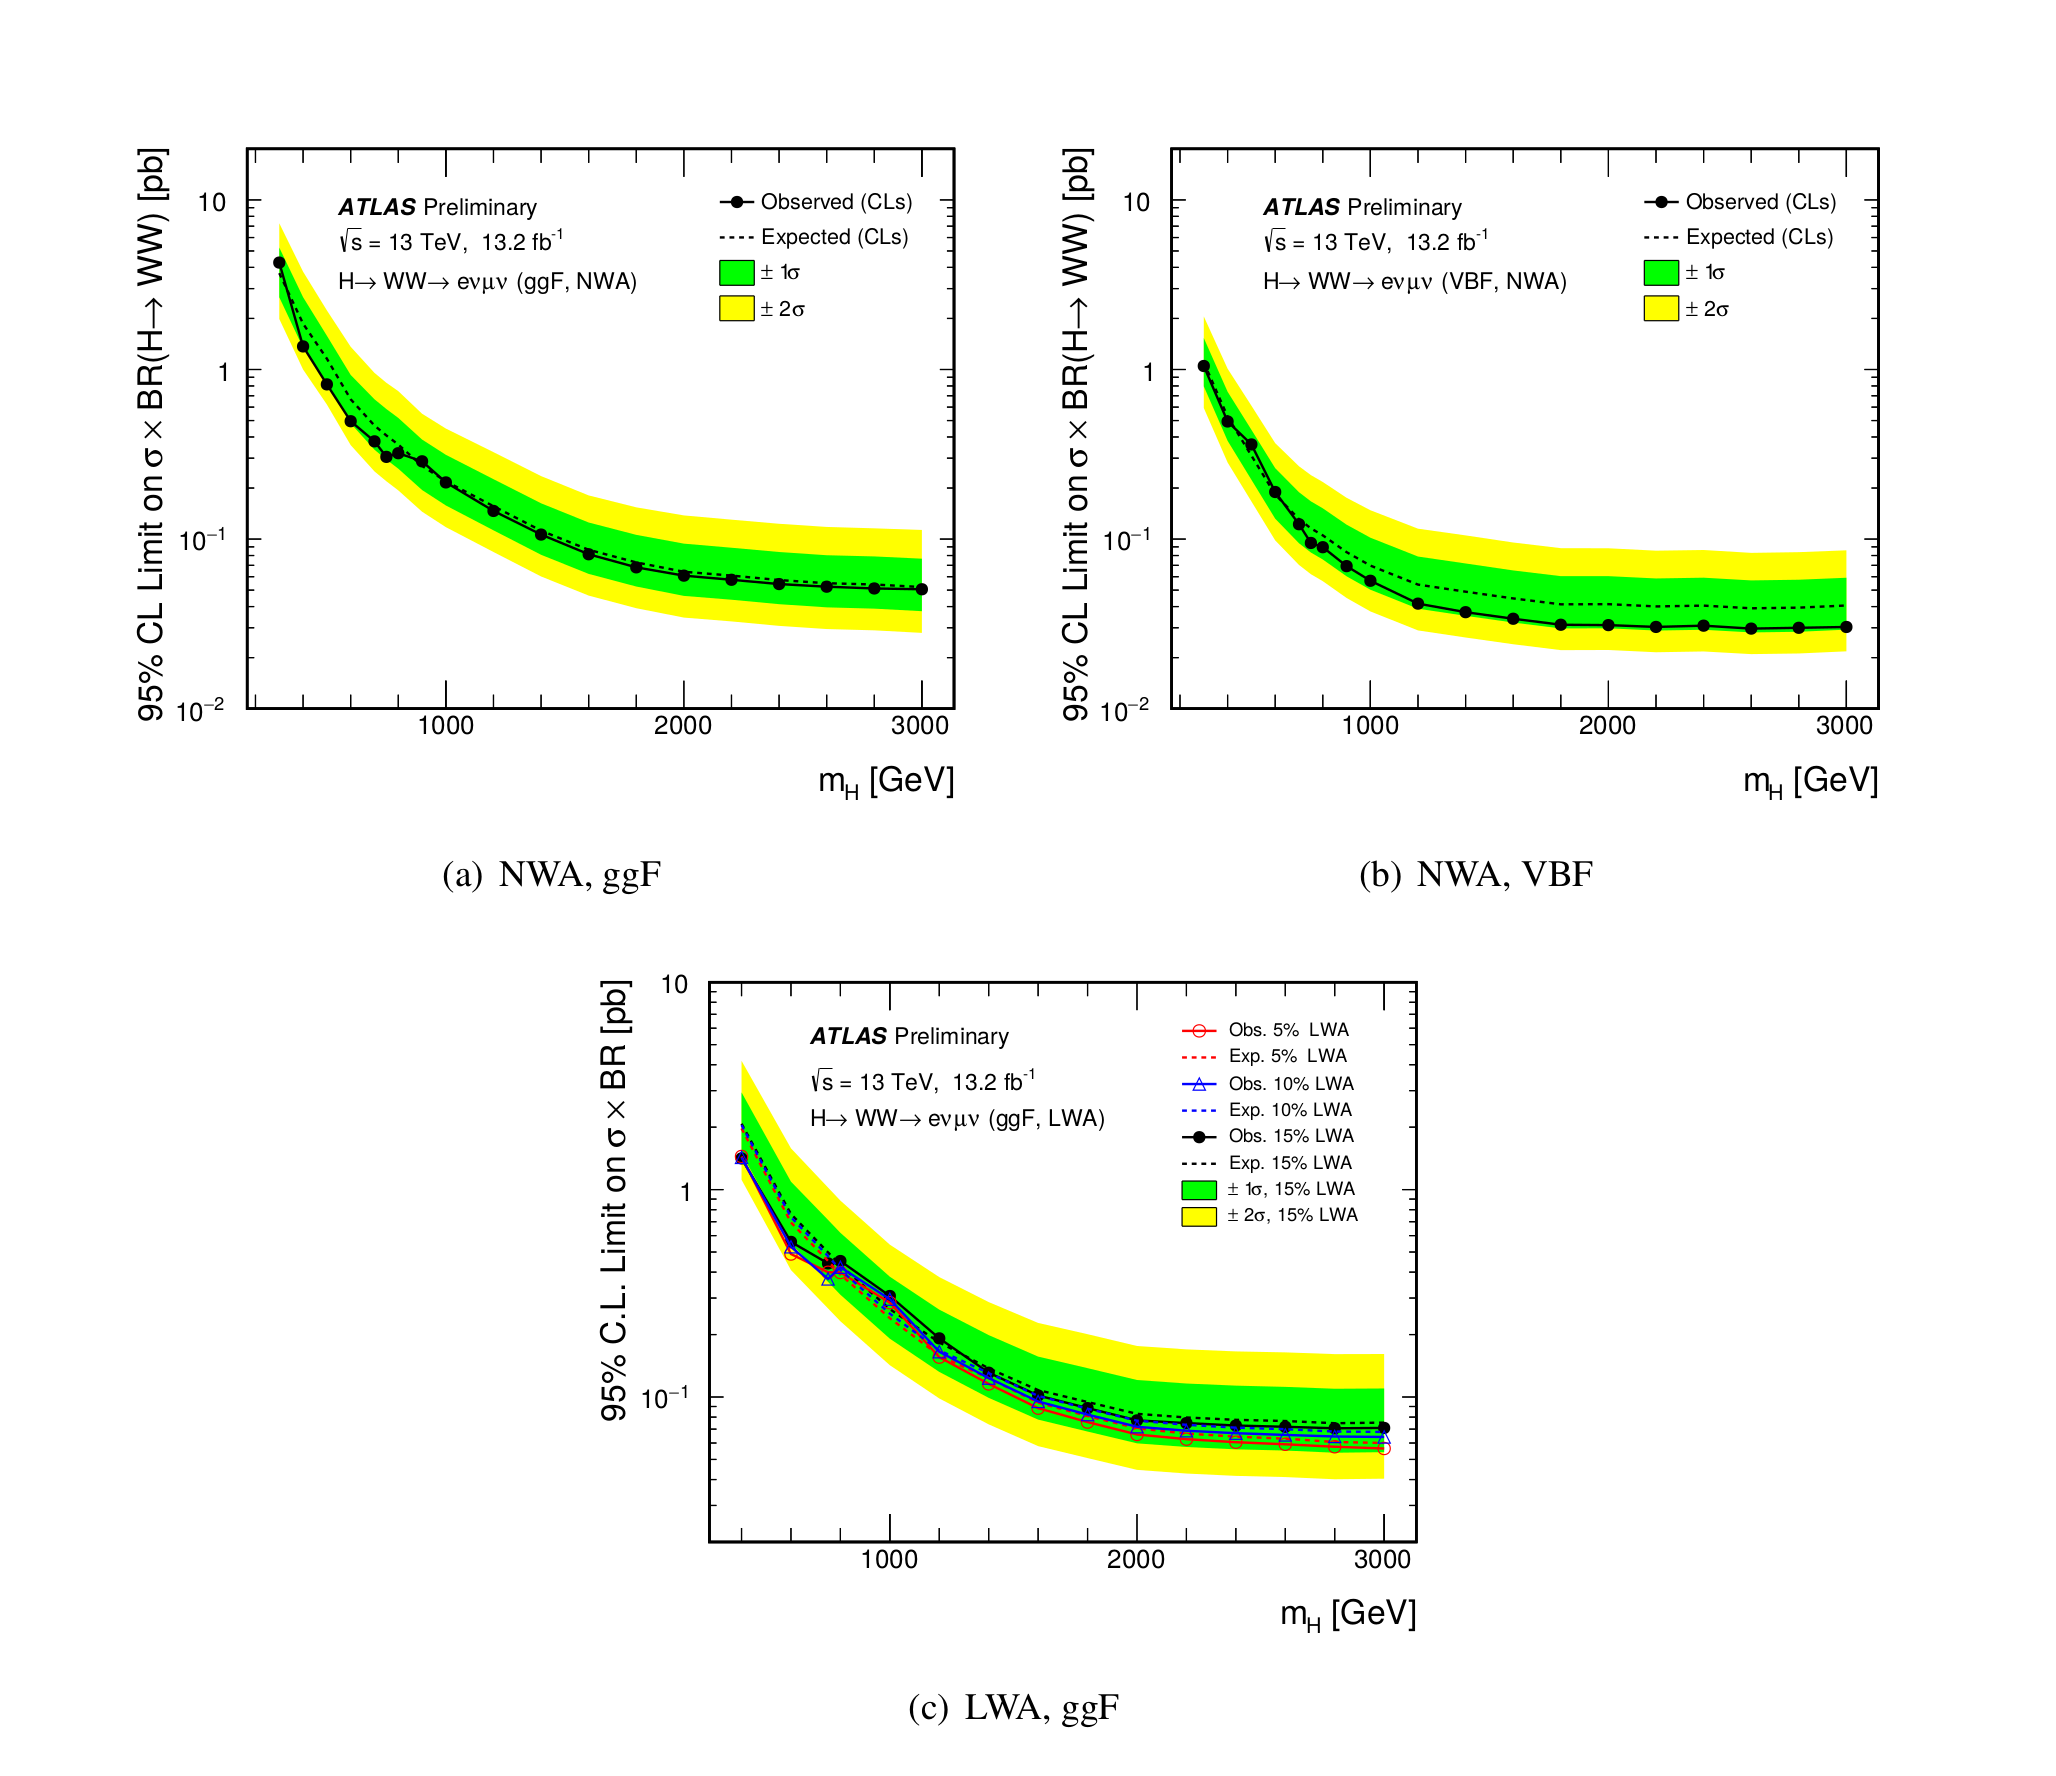
\includegraphics[scale= 0.9]{../Cap1/ATLAS-CONF-2016-074}
\caption{95\% CL upper limits on the Higgs production cross section times branching ratio in the analysis, for signals with narrow-width (gluon gluon fusion or VBF) in the top row and the 5\%, 10\% and 15\% width lineshapes (gluon gluon fussion only) in the bottom. The green and yellow bands show the  $\pm 1\sigma$ and  $\pm 2\sigma$ uncertainties on the expected limit. }
\label{ATLAS-CONF-2016-074_fig}
\end{figure}
